\chapter{User-Driven Structure Design to Support Real World Objects}

\begin{figure} [h]
   \centering
   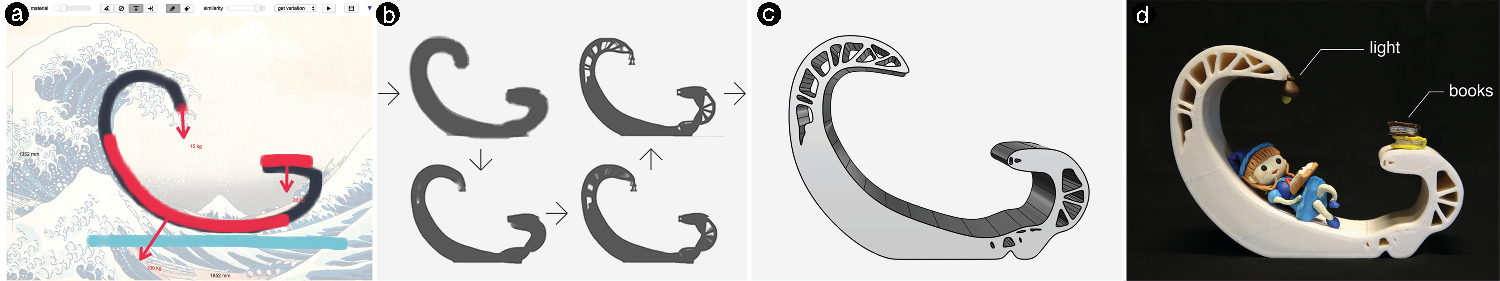
\includegraphics[width=1\textwidth]{figures/kanagawa}
   \caption{Forte is a 2D design tool that takes a user-driven approach of generative design: a user sketches a reading chair inspired by the  painting `The Great Wave off Kanagawa' (a) with specified loading scenario (red arrow forces, blue ground); Forte then generates structures (with real-time feedback) to support the loads while resembling the user's sketch (b), which can then be post-processed to create a 3D fabrication-ready model (cd).}~\label{fig:fig1}
\end{figure}

In both of the previous projects---Encore and Reprise, the design task is based on an existing object and the outcome is some sort of extension that enhances a specific function of that object. While this approach works for creating something incremental (e.g., adaptation), it becomes problematic when scaling up---creating self-contained objects such as bookshelf, step stool, or wine rack.

There are several challenges in designing this class of objects. Foremost, as they are no longer incremental add-ons to existing objects, it would be difficult to create a design \textit{in situ} from these real world objects. Consider making a bookshelf for example. It is less straightforward if one has to start the design with some books; rather, a more intuitive approach is the reverse: create the bookshelf first, then see if it has enough space, or is strong enough to accommodate the books. However, for non-expert users, it is hard to create a functional design by intuition. A user might have an intuition about what their bookshelf should look like, and might be able to sketch the design; but they would probably have trouble making sure that this design would work---that is, supporting all the books to be put on it.

To ensure that a design meets such functional requirement, generative design methods such as \textit{topology optimization}
% \footnote{While `generative design' refers to a broader set of approaches, we focus on the one using topology optimization. The remainders of the paper will use these two terms interchangeably.} 
will automatically optimize material distribution given the constraints of space, material amount and other functional requirements \cite{sigmund200199}.
% =======
% Traditionally, to solve such problems, methods such as topology optimization will automatically optimize material distribution given the constraints of space, material amount and other functional requirements \cite{sigmund200199}.
% >>>>>>> 994990b10e609aa6dd81e7dd787c074591ca4222
Though promising, such methods provide very few ways for users to directly express or manipulate their designs; instead, users have to map their design ideas--often unintuitively--to mathematical input parameters. Further, it is often assumed that a CAD model has been designed prior to using such methods. As a result, there is a lack of support for users' ideation process, and they have little direct control of the optimization's outcome \cite{zhou2016direct}, or ways to effectively iterate their designs.

To address this problem, prior work and existing tools have been focusing on interactively specifying the input parameters \cite{aage2013interactive, Stressto43:online}, adding template-based textures to the optimized results \cite{martinez2015structure}, or contextualizing them with CAD \cite{shea2003towards} or freeform sketching \cite{kazi2017dreamsketch}. However, none of this work lets users directly control how a design should be generated and optimized.

%  \cite{aage2013interactive} and a few existing tools \cite{Stressto43:online} have sought to enable users to spatially manipulate the input parameters, which updates the optimization accordingly; however, this still gives users only indirect control over the results.
% % one approach is to let users provide a 3D model and optimize it while keeping it similar to the original shape \cite{zhou2016direct}. This, however, assumes users already have a fully designed object in mind. 
% Another solution is to directly specify the appearance of the optimized structure by providing examplar visual patterns \cite{martinez2015structure}, which, however, only focuses on low-level textures rather than high-level look-and-feel. To give users more freedom of control, a third approach is to create fabricatable objects via sketching \cite{igarashi2007teddy}; however, often users are not sketching the parts to be optimized \cite{kazi2017dreamsketch}, or when they do there is little direct guidance on improving the sketch for better performance \cite{saul2011sketchchair}. 

% sketch chair
% martinez
% zhou
% !!! stress relief

%Technical Solution
To help address these issues, we present Forte, a sketch-based 2D design tool that takes a user-driven approach for people to directly express and iterate on their ideas through generative design with real-time visual feedback.
%Contribution
Our main contribution is a technical approach that supports a high-level dialog allowing a simpler expression of users' design intent, resulting in a combination of structural performance and less quantifiable objectives to be achieved in the results. Figure~\ref{fig:fig1} shows an exemplar workflow: sketching a reading chair inspired by the famous painting `The Great Wave off Kanagawa'\footnote{\url{https://en.wikipedia.org/wiki/The_Great_Wave_off_Kanagawa}} with a specified loading scenario; Forte then generates structures to support the loads while resembling the user's sketch, which can then be post-processed using external tools (e.g., Rhinoceros) to create a 3D fabrication-ready model.

Specifically, with Forte, users can ask the system to add structures to the original sketch, provide a variation with better performance, or generate optimized internal structures.
Users can globally adjust a `similarity' slider, which controls how much the system will `deviate' from their initial input; they can also locally edit the design by adding or erasing parts of the sketch, which then interactively prompts the system to update based on this new information.
 % while informed of the performance trade-off by a visualization.
Meanwhile, a visualization informs users of the performance trade-off as they iterate on the design.
Building on a fast topology optimization engine \cite{andreassen2011efficient}, Forte enables rapid iteration and exploration, unlike most existing practices that run the process in a non-interactive, batch fashion (even for 2D designs).

\begin{figure*} [t]
  \centering
  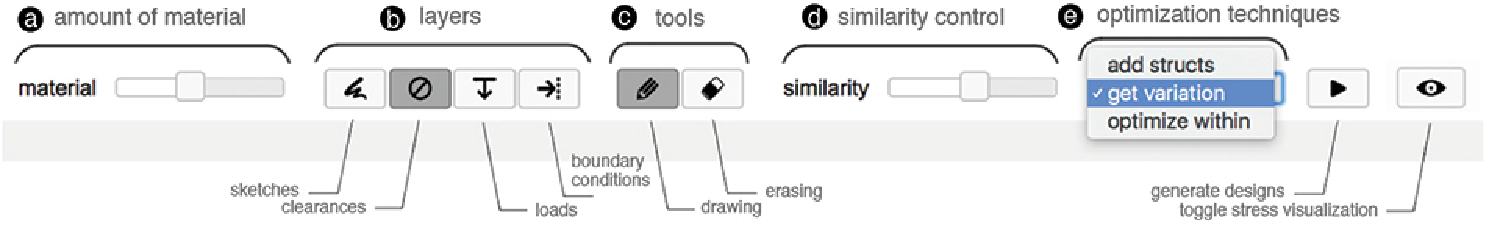
\includegraphics[width=1\textwidth]{figures/overview}
  \caption{Overview of Forte's default tool bar: adjusting the amount of material for generating the structures (a); different layers for sketching and specifying the loading scenario (b); drawing and erasing tools (c); controlling how the generated results are similar to the original sketch (d); and selecting different design optimization methods (e).}~\label{fig:overview}
\end{figure*}

%Validation
We envision Forte will empower professionals who design structures, such as industrial designers, mechanical engineers and architects. To validate our approach, we held design sessions with 10 participants. Our study demonstrates that Forte empowers designers to create and explore a range of optimized designs with custom forms and styles. While our current focus is on a 2D design tool, we showcase three post-processing techniques using external tools to turn a 2D design to a 3D object: \textit{extrusion}, \textit{warping} and \textit{combination}. We report stress analysis on these 3D models under varying loading conditions and finally demonstrate a series of fabricated examples.


\begin{figure} [h]
  \centering
  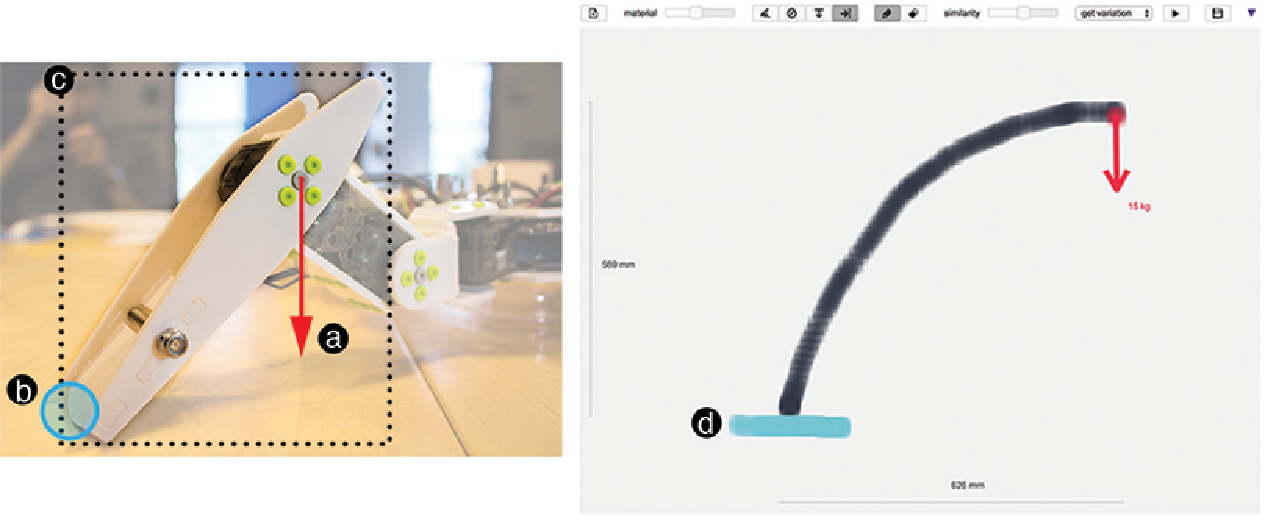
\includegraphics[width=0.75\textwidth]{figures/design_scene}
  \caption{From users' sketch, Forte (right) generates lightweight structures to support loads, such as a robot leg (left) that needs to support the robot's weight using a specified amount of material.}~\label{fig:design_scene}
\end{figure}

\section{Forte: User-Driven Generative Design}

\begin{figure*} [t]
  \centering
  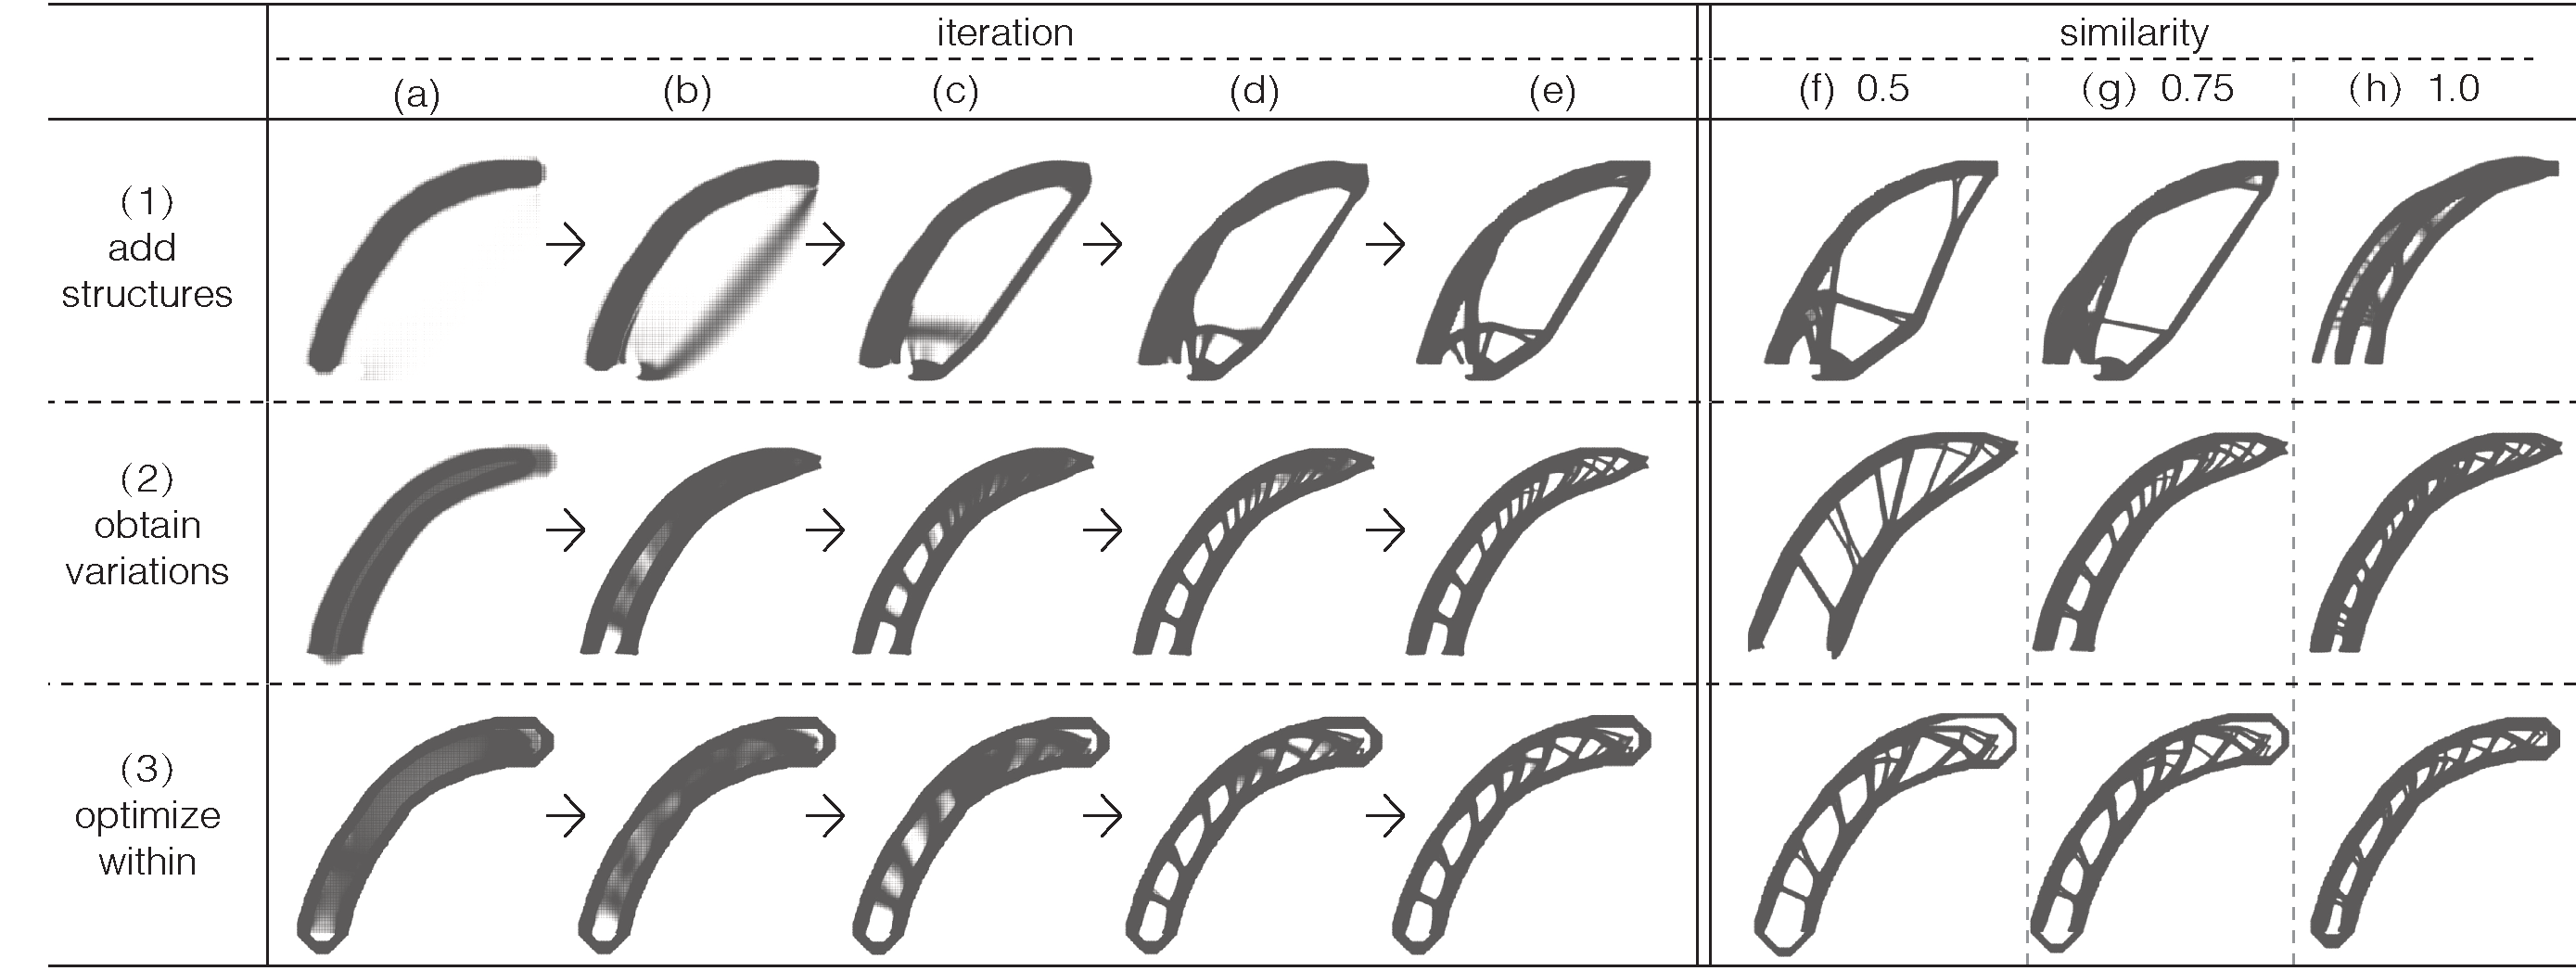
\includegraphics[width=1\textwidth]{figures/all_the_techniques}
  \caption{Forte's three types of design optimization iteratively generate structures based on user's sketch while providing them with real-time visual feedback akin to an animiation (a-e), the result of which can be controlled by a global `similarity' value (f-h).}~\label{fig:techniques}
\end{figure*}

In this section, we describe users' interaction with Forte and its key features for user-driven generative design, while leaving the technical details for later in the next section. Specifically, we will walk through a usage scenario: creating a 2D design of a leg for a quadruped robot (Figure~\ref{fig:design_scene}). The design goal is three-fold: {\em (i)} in contact with the ground (Figure~\ref{fig:design_scene}b), the leg needs to be optimized for supporting the weight of the robot's body (Figure~\ref{fig:design_scene}a), {\em (ii)} it needs to be lightweight to ensure the overall efficiency of the robot, and {\em (iii)} its form also needs to be customized with respect to other user-defined goals such as aesthetics. Below we first go through some basic concepts and terminologies and then demonstrate how Forte allows users to jointly achieve these goals.

\subsection{Basic Concepts and Terminologies}
Generative design via topology optimization considers an object as a distribution of a certain amount of material in order to meet certain performance criteria. This paper focuses on structural performance, which is optimizing structures---with only a limited amount of material available---to support a given load. For instance, a robot leg should be designed to support the weight of the robot's body with a lightweight structure. In Forte, a design consists of a sketch (considered below) and a \textbf{loading scenario}, which include {\em(i)} where the expected \textbf{loads} are and how large they are, and {\em(ii)} \textbf{boundary conditions}, which is where the object is in contact with its environment (e.g., a robot leg will touch the ground, as shown in Figure~\ref{fig:design_scene}). Based on this input, Forte will then generate structures via different types of \textbf{design optimization}, i.e., distributing allocated material in a structurally optimized way. Each type of optimization is also constrained by a given \textbf{amount of material}, which is typically measured by the percentage of the entire \textbf{design domain}--the bounding box of the design object (Figure~\ref{fig:design_scene}c). For example, 30\% material means the material used for the robot leg amounts to 30\% the size of its bounding box\footnote{We discuss later in the design sessions that participants found this to be a problematic way of measuring material, as it seems hard to get an intuitive estimate based on bounding boxes.}.

\subsection{Sketching Designs and Loading Scenarios}
With Forte, a user sketches a design idea as well as the loading scenario. Each type of sketch is drawn in a different color on its own layer (Figure ~\ref{fig:overview}b). This allows users to select and focus on one particular layer at a time. Once a layer is selected, it is pushed to the top with the rest of the layers set to semi-transparent.

\begin{figure} [h]
  \centering
  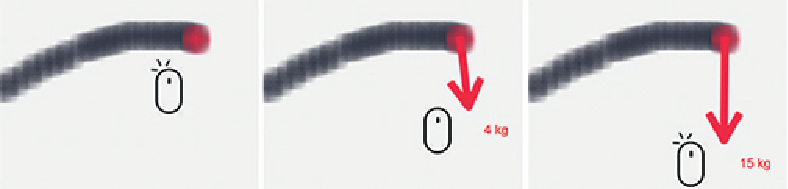
\includegraphics[width=0.7\textwidth]{figures/draw_load}
  \caption{Interaction to specify a load.}~\label{fig:draw_load}
\end{figure}

To start, a user simply selects the design layer and sketches a curve representing the robot's leg. With Forte, it suffices to provide such a simple representation that succinctly expresses the user's high-level design intent, i.e., ``I want the robot's leg to curve like this''. As the user sketches the robot leg, Forte also shows the dimensions of the current sketch's bounding box to inform users of the size of their design. The default scale is 20 mm per pixel, which can also be adjusted by the user in the preference settings.

As a next step, the user would consider the loading scenario. First, to create a load, the user switches to the load layer (Figure~\ref{fig:overview}), They can click on the sketch to indicate a single loading point, or draw to specify a sequence of loading points. As shown in Figure~\ref{fig:draw_load}, as soon as these points are drawn (e.g., mouse released), an arrow is rendered, following the cursor (e.g., where the mouse moves), and indicating the direction as well as the amount of load, which is also shown at the end of the arrow. A click confirms and pins down this load vector. To specify a boundary condition, the user simply draws it on the corresponding layer (Figure~\ref{fig:design_scene}d).

In addition, Forte also supports a fourth type of layer that allows users to lasso-select a \textbf{clearance} region that needs to be kept clear, e.g., the space above a chair's seat or around the tip of a hook (Figure~\ref{fig:draw_clearance}). This information proactively prevents generating structures at places that will compromise the usage of an object.

\begin{figure} [h]
  \centering
  \vskip 4pt
  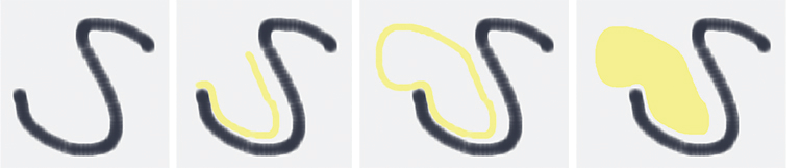
\includegraphics[width=0.7\textwidth]{figures/draw_clearance}
  \caption{Lasso-selecting an area of clearance around the tip of the hook (no structure generated here).}~\label{fig:draw_clearance}
\end{figure}

\begin{figure*} [t]
  \centering
  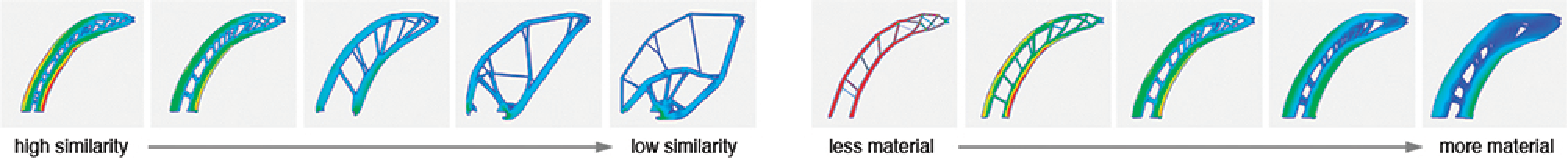
\includegraphics[width=1\textwidth]{figures/sim_mat}
  \caption{Stress visualization informs performance trade-off between different similarity values (left), and the amount of material (right).}~\label{fig:sim_mat}
\end{figure*}

\begin{figure*} [t]
  \centering
  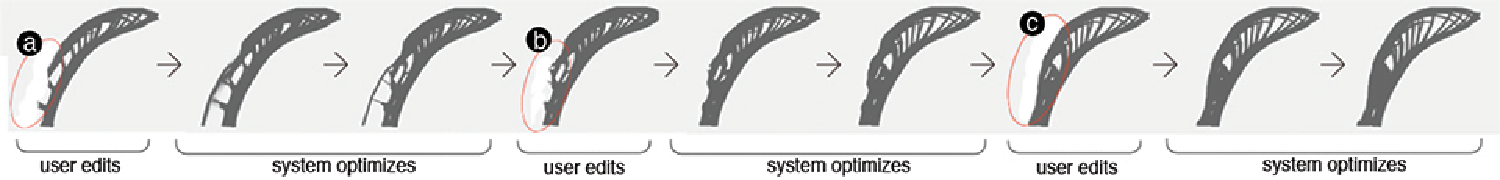
\includegraphics[width=1\textwidth]{figures/local_editing_eraser}
  \caption{Users can suggestively erase part of a generated result (ab), which prompts the system to update the optimization addressing the intent of removing material; with this tool, users can also refine or smoothen a generated result (c).}~\label{fig:local_editing_eraser}
\end{figure*}

\subsection{Design Optimization with Global Similarity Control}

Once the user creates a sketch and specifies the loading scenario, they can now explore three different ways the system can generate structures by design optimization. Forte considers the generation of structures  as a spectrum between users' original idea and the system's solution to the defined problem. Users can navigate on this spectrum by adjusting a \textit{similarity} value from 0 to 1 (Figure~\ref{fig:overview}d): conceptually, a low similarity would allow the system to `deviate' more from the user's initial sketch while a higher value will keep the generated structures closer to what the user originally draws. Further, Forte's optimization algorithms run at an interactive rate, providing users with real-time visual feedback after each iteration, as demonstrated in the accompanying video figure.
% As shown in Figure \xx, a design with $375\times323=121,125$ finite elements can be generated in less than two minutes. 
Below we illustrate Forte's three new generative design optimizations and how similarity allows users to have direct control of the generated results.

% \begin{figure*} [t]
%   \centering
%   \includegraphics[width=2\columnwidth]{figures/gv_similarity}
%   \caption{Obtain variations: as similarity increases (a$\rightarrow$e: 0, 0.25, 0.5, 0.75, 1.0), generated variations follow the user's sketch more closely; turning on the stress visualization shows the structural tradeoff.}~\label{fig:gv_similarity}
% \end{figure*}

\textbf{Add structures} \hspace{0.1cm} To start, Forte can generate additional structures to strengthen the user's original sketch. For example, as shown in Figure~\ref{fig:techniques}(1a-1e), a major truss structure is added parallel to the user-sketched robot leg as reinforcement. 

%\begin{figure} [h]
%  \centering
%  \includegraphics[width=1\columnwidth]{figures/add_structs}
%  \caption{Add Structures: generating additional structures (a$\rightarrow$e) for the robot leg to strengthen the user's original sketch (this trial: 121,125 elements, 30 iterations, 3.45 sec. per iteration).}~\label{fig:add_structs}
%\end{figure}

The similarity value effectively controls how far away from the original sketch these structures can be added. As the user increases similarity, added structures will appear increasingly closer to the original sketch and eventually become part of it, equivalent to a thickening operation (Figure~\ref{fig:techniques}(1h)). However, note that the added structures' position does not change smoothly with the similarity value; rather it tends to `snap' to positions along the way that are structurally meaningful. 
% SEH: seems ok to me \xac{not sure the last sentence is understandable}

Overall, `add structures' is targeted at situations where users only have a partial or incomplete design idea in mind and are unsure whether and how they should add extra structures to provide support for the loads.

%\begin{figure} [h]
%  \centering
%  \includegraphics[width=1\columnwidth]{figures/as_similarity}
%  \caption{Add structures: as similarity increases, added structures emerge closer to the original sketch (similarity value a$\rightarrow$e: 0.5, 0.75, 1.0). }~\label{fig:as_similarity}
%\end{figure}

\textbf{Obtain variation} \hspace{0.1cm} Forte provides a second optimization algorithm that can generate variations of the initial sketch. For example, as shown in Figure~\ref{fig:techniques}(2a-2e), Forte generates two parallel interconnected trusses instead of one user-sketched structure; however, the variation still bears resemblance to the original sketch as it globally follows the curve path specified by the user. As the user increases the similarity value, the generated structures will follow the user's sketch more closely (Figure~\ref{fig:sim_mat}). `Obtain variation' works best when users only have a concept (e.g., a skeleton) of what the design should look like without any structural details, in which case the system will take the initial designs as `seeds' and vary it with generated structures.

%\begin{figure} [h]
%  \centering
%  \includegraphics[width=1\columnwidth]{figures/get_variations}
%  \caption{Obtain variations: generating a variation (a$\rightarrow$e) of the initial sketch to improve the structural integrity (this trial: 121,125 elements, 30 iterations, 2.91 sec. per iteration)}~\label{fig:get_variations}
%\end{figure}

\textbf{Optimize within} \hspace{0.1cm} Forte can also consider the user's sketch as solid shapes (rather than skeletons) and optimize the internal structures within. For example, as shown in Figure~\ref{fig:techniques}(3a-3e), Forte reproduces the contour of the user-sketched robot leg while filling in generated structures. By controlling similarity, the user can effectively shrink or expand the contour, e.g., decreasing similarity results in a robot leg of the same curvy shape but much thicker than the original sketch, given the system more space to generate structures. `Optimize within' serves well for cases where users already have a fully-designed solid shape but want to re-design the interior structures.

%\begin{figure} [h!]
%  \centering
%  \includegraphics[width=1\columnwidth]{figures/optimize_within}
%  \caption{Optimize within: expanding user sketch into a contour and generating (a$\rightarrow$e) internal optimized material layout (this trial: 121,125 elements, 30 iterations, 2.87 sec. per iteration).}~\label{fig:optimize_within}
%\end{figure}
%
%\begin{figure} [h!]
%  \centering
%  \includegraphics[width=1\columnwidth]{figures/ow_similarity}
%  \caption{Optimize within: lowering similarity expands the contour of the user sketch, allowing more room for optimization to generate structures (similarity value a$\rightarrow$c: 3.5, 5, 7.5).}~\label{fig:ow_similarity}
%\end{figure}

For any of these design optimizations, users can adjust how much material can be used in generating the design. For example, as shown in Figure~\ref{fig:sim_mat}, reducing the material amount often creates hollow structures with trusses, while a higher value tends to thicken or fill up certain parts of the design.

% \begin{figure*} [t]
%   \centering
%   \includegraphics[width=2\columnwidth]{figures/gv_material}
%   \caption{Reducing the material amount often creates hollow structure with trusses, while a higher value tends to thicken or fill up certain parts of the design (amount of material a$\rightarrow$e: 5\%, 10\%, 15\%, 20\%, 25\%).}~\label{fig:gv_material}
% \end{figure*}

As the user runs one of the three optimizations, Forte creates and records a trial, and together displays a history of results from all these trials. Selecting a trial not only shows the resulted structures, but also updates the menu so that users can see which of the three optimizations was used, how much material was allocated and what similarity value was applied.


\begin{figure} [b]
  \centering
  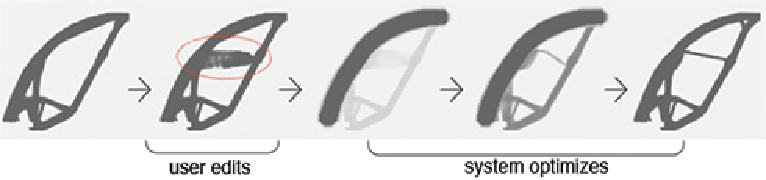
\includegraphics[width=0.75\columnwidth]{figures/local_editing_pencil}
  \caption{Users can suggestively add material to a generated result (circled strokes), which prompts the system to re-run the optimization and attempt to add structures accordingly.}~\label{fig:local_editing_pencil}
\end{figure}

\subsection{\#3 Refining Optimization with Local Suggestive Edits}
The similarity value allows users to control the optimization outcome at a global level with respect to the entire design. Complementarily, once a result is generated, users can also perform fine local editing, which will prompt the system to re-run the optimization, taking into account users' underlying intent of the edit. For example, if a user wants a thinner tip of the robot leg, they can use the eraser tool (Figure~\ref{fig:overview}c) to scrub that area (Figure~\ref{fig:local_editing_eraser}a, shadowed part). The system immediately starts a new optimization and returns an updated result with less material on the tip of the leg. Increasing the erasing `power' and applying it again finally sharpen the leg, but results in a rough outline (Figure~\ref{fig:local_editing_eraser}b). We can also use this tool to smooth the optimized result (Figure~\ref{fig:local_editing_eraser}c).

Similarly, the user can also use the pen tool (Figure~\ref{fig:overview}c) to draw on an optimization result, such as adding a truss to the leg (Figure~\ref{fig:local_editing_pencil}ab). The system will also re-run the optimization and will attempt to generate some structures where the new truss is drawn (Figure~\ref{fig:local_editing_pencil}).

This technique is called suggestive editing, as users' action do not directly remove or add to the design; rather, it serves to suggest their intent to the system, e.g., ``I want less material here'', or ``I would like to add something there''. The next round of structure generation will take into account such intent and attempt to realize it through the optimization process. However, intent cannot be realized if the removal or addition of material compromises the structural integrity of the design (e.g., removing the entire bottom part of the robot leg, making it unable to stand on the ground).

\subsection{\#4 Informing Performance Trade-offs with Visualization}
As users exploratively customize the optimization process, it is important to inform them of the performance trade-offs. Forte allows users to toggle a stress visualization (Figure~\ref{fig:overview}) overlaying each optimized result (Figure~\ref{fig:sim_mat}) . The heat map indicates which part of a design is the weakest; it also allows users to compare different designs' performance and see how the stress situations evolve as the design evolves. Users can also adjust the safety factor: a higher value is equivalent to assuming more weight, thus revealing more structurally problematic areas in the design.
 
% \pagebreak

\section{Implementation}
In this section we describe technical details of Forte's implementation. 

\subsection{Sketching Designs and Loading Scenarios}
Recall that users' design input consists of a sketch within a design domain as well as loads, boundary conditions (Figure~\ref{fig:design_scene}), and/or clearance (Figure~\ref{fig:draw_clearance}).

Given these input parameters, first the design domain is discretized into $N=W \times H$ square \textbf{finite elements} \cite{zienkiewicz1977finite}, each of which (denoted as $e$) is assigned a \textbf{density} value $x_e \in [0, 1]$. The user's intial sketch is discretized into a binary density map on this domain with 1's for elements overlapping with the sketch and 0's for the others. Similarly, loads, boundary conditions and clearance are also converted to such density maps.  In addition, for loads each density=1 element is also associated with a load vector indicating the amount of the load as well as the direction. 

% Specifically, if users draw a sequence of load points, we divide the load vector across all the points so that $\Sum{\mathbf{n}_j \dot \mathbf{f}_j}/=\mathbf{f}$, where $\mathbf{n}_j$.
%
% \xac{explain why fitting circle}

\subsection{Design Optimizations with Global Similarity Control}
The implementations of the three design optimization techniques presented here are developed based on the 88-line program \cite{andreassen2011efficient}, which uses a SIMP (Solid Isotropic Microstructure with Penalization) method for topology optimization. For readers to better understand our approach, we first provide a brief of overview and refer the reader to Andreassen et al. for further details \cite{andreassen2011efficient}.

Overall, the process solves the following compliance optimization problem:
\begin{equation}
	\min_x: c(\mathbf{x}) = \mathbf{U}^T\mathbf{K}\mathbf{U} = \sum^N_{e=1} E_e(x_e)\mathbf{u}_e^T\mathbf{k}_0\mathbf{u}_e,\\
\end{equation}
	subject to:
\begin{gather*}
	{V(\mathbf{x}) / V_0} \leq f ; ~~ 
	\mathbf{K}\mathbf{U} = \mathbf{F};  ~~
	0 \leq x_e \leq 1
\end{gather*}
where $c$ is the compliance of the design, which is computed with $\mathbf{U}$ -- the global displacement matrix, and $\mathbf{K}$ -- the global stiffness matrix determined by the stiffness of the material as well as its distribution (or layout). The objective function is further broken down to the summation of compliances across all elements: $E_e$ is the Young's modulus of $e$ ($E_e = E_{min} + x_e^p(E_0 - E_{min})$), $\mathbf{k_0}$ is the unit stiffness matrix which together with $E_e$ determines the stiffness of element $e$; $u_e$ is the displacement vector of $e$. Finally, $\mathbf{U}$ can be computed from $\mathbf{K}\mathbf{U} = \mathbf{F}$, where $\mathbf{F}$ is vector of forces (loads).

% \begin{equation}
% x_e^{new} = optimize(x_e) = {{1 \over {\sum_{j \in N_e}{H_{ej}}}}} \sum_{j \in N_e}{H_{ej}x_e}
% \label{eq:opt_xe}
% \end{equation}

At each iteration, once $c$ is computed, $x_e$ is updated as follows:
\begin{equation}
% \begin{aligned}
	x_e^{new} = 
	\begin{cases}
    max(0, x_e-m),	& \text{if } x_eB_e^\eta \leq max(0, x_e-m) \\
    min(1, x_e+m),  & \text{if } x_eB_e^\eta \geq min(1, x_e-m) \\
    x_eB_e^\eta 	& \text{otherwise}
	\end{cases}
% \end{aligned}
\end{equation}
where $m$ is a pre-set step for density changes, $\eta = 1/2$ is a numerical damping coefficient, and $B_e = (-{\partial c \over \partial x_e})/(\lambda{\partial V \over \partial x_e})$, with $\lambda$ being a constraint factor to ensure the total volume does not exceed $V_0f$---the allocated amount of material where $f$ is the percentage and $V_0$ is the volume of the design domain.

% cite: stress relife; guided exploration
% \subsection{Types of Design Optimizations with Controlled Similarity}
% [figure] the part of the ui with the three options

This process represents the classic topology optimization approach that automates the generation of structures in a `black box'. Below we describe our methods of extending it to a user-driven approach, allowing the control of the optimization results via a similarity value.


\textbf{Add structures} \hspace{0.1cm}
We initialize the design domain by assigning each element the value of $f$
%the specified amount of material 
(e.g., 15\% of the bounding box area). Through iterations the optimization will increase or decrease this value for a given element, thus forming a global structure. After each iteration, we add the intermediate generated structures to the user's sketch, and take it as the input for the next iteration. Specifically, now each element density is computed as
\begin{equation}
    \widehat {x_e^{new}}= 
\begin{cases}
    1,          & \text{if } e \in user~sketch\\
    x_e^{new}	& \text{otherwise}
\end{cases}
\end{equation}
To control similarity, we perform a \textit{mass transport} (cf. \cite{bonneel2011displacement}) after each iteration before adding the intermediate results to the user's sketch. A mass transport considers two designs (e.g., user sketch vs. optimized result) as two ways of distributing the same amount of mass (computed by summing up elements' density), and transports the mass in between the two distributions to obtain an interpolation. We use mass transport to interpolate between the optimized result and the user sketch, taking similarity as the weight of interpolation (0: user sketch --- 1: optimized result). This allows us to control how much the design will be similar to the original sketch after adding the optimized result.

We implement the mass transport function by computing and interpolating the barycenters of the two input designs as distributions. We compute the distance field of the user sketch and use it as the input distribution to the mass transport function. This provides more fine-grained information at each element (what is the distance of this element to the user sketch) beyond a binary value (whether or not it is part of the user sketch).

\textbf{Obtain variation} \hspace{0.1cm}
Instead of $f$, we initialize the design domain with the user's sketch, and then run topology optimization, which will effectively `shift' the material away from user-specified locations to achieve a variation with optimized material layout.

%To control similarity, we first experimented with the same mass transport approach. However, it tends to `oscillate' between user sketch and the optimized result, and takes long to converge. Before this problem did not occur, which we hypothesize is because it is operating on a smaller `delta' between user sketch and optimized result (at n+1 th iteration, the result is optimized from the n th iteration's added to user sketch). 
%
%Thus we take a different approach, focusing on controlling similarity right from the input. Specifically, we map the distance field of the user's sketch to the input design domain as 
To support user control of similarity,  we map the distance field of the user's sketch to the input design domain as 
\begin{equation}
x_e^{initial} = {1\over \sum_{i=1}^N{cos({{\pi d(i)}\over 2})^s} }cos({{\pi d(e)}\over 2})^s f
\end{equation}

where $x_e^{initial}$ is the initial material density at element $e$, $d$ is the normalized distance field function, $s$ is the user specified similarity request, and the $cos$ function raised to $s$ produces value close to 1 when $d(e)$ is small (close to the user's sketch) and drops rapidly to 0 when shifting away. $s$ controls how quickly such a drop occurs. Thus a larger similarity value will initialize the optimization (hence the result as well) more closely to the user's sketch, while a smaller value will loosen the constraint by `diluting' the user's sketch, and produces a result with wilder variation.

% One limitation of this approach is that if part of the user's sketch is considered `unnecessary' (i.e., not providing structural support), the optimization will tend to reduce a larger chunck of it, resulting a disproportional dissimilarity to the original design. To provide an alternate approach which avoids this problem, we introduce the following method that always keeps the shape of the user's sketch and optimizes the structure within.

\textbf{Optimize within}
We consider the user's sketch as a `skeleton'. As a first step, we expand it using the distance field by setting a new contour around the original sketch. We then run the optimization only within the contour, as follows, at each iteration,
\begin{equation}
    \widehat {x_e^{new}}= 
\begin{cases}
    x_e^{new},	& \text{if } d(e) < d_c\\
    1,              		& \text{if } d_c \leq d(e) < d_c + t\\
    0 						& \text{otherwise}
\end{cases}
\end{equation}
$d_c$ is a distance field value used to define the new contour, and $t$ controls the thickness of the contour. We control similarity by shifting $c$ towards or away from the user's original sketch.

% \textbf{Comparing the three design optimizations}
% ...

% \subsection{Controlling Global Similarity}

\subsection{Refining Optimization with Local Suggestive Edits}
% As users perform the initial sketch and run it through the above design optimization, they might expect to edit the results. 
Forte enables users to interactively suggest adding to, or removing from, parts of the optimization result, which then prompts the system to re-run the optimization to produce a version that matches the users' intent, including the new edits. Importantly, in such re-run, the system is initialized based on the result from the previous run, rather than starting from the original sketch.

As a user draws on, or erases, parts of a design on a $W \times H$ domain, we create a mask $M$ of the same dimensions with each pixel's value $M_e \in [1-\Delta_{remove}, 1+\Delta_{add}], \Delta_{remove} \in (0, 1), \Delta_{add} > 0$. Then in the optimization process, we update element $e$ as
\begin{equation}
\widehat {x_e^{new}}=M_e x_e^{new}
\end{equation}
In essence, $M_e$ indicates whether and how much a user would want to add or remove material at this point.
% \begin{equation}
%     x_e^{new}=M_e \, optimize(x_e)
% \end{equation} 
If a user performs an erasing action, $M_e$ is set to be in $[1-\Delta_{remove}, 1)$, which will dampen the to-erase elements' density at each iteration; if a user performs additional drawing, we integrate the addition to the result as input for the re-run. As $M_e$ is now set to be in $(1, 1+\Delta_{add}]$, it will amplify the to-add elements' density at each iteration. All unedited $M_e$'s will be set to 1.

% Further, we also allow users to control whether to erase or add material percisely at some locations, or more loosely in a certain area. This is enabled by smoothing $M$ using a variable Gaussian kernel. 

\subsection{Informing Performance Trade-offs with Visualization}
We compute the von Mises stress of each optimized result using Biyikli and To's method \cite{biyikli2015proportional}, which is implemented as an integral component of the optimization process. The values in the stress distribution are then normalized by a material-specific yield stress $\sigma_y$ and visualized as a heat map. All our examples and demonstrations in the design tool use a material model based on an Extrusion Grade PLA \cite{NatureWo45:online}. The yield stress is also divided by the user-specified safety factor, e.g., a $2\times$ safety factor will result in the use of $\sigma_y/2$, thus visually revealing more potentially problematic area in the design.

\subsection{Software and Hardware}
The front end of Forte is written in JavaScript using jQuery\footnote{jQuery: \url{https://jquery.com/}} for UI development. The back end consists of two components: {\em(i)} the optimization techniques were written in MATLAB, which is then compiled into a standalone service; and {\em(ii)} a phython-based server which relays optimization requests and input parameters from the front end to the MATLAB service, and sends back the results. Everything runs on a MacBook Pro (Retina, 15-inch, Early 2013) with a 2.4 GHz Intel Core i7 and 8 GB 1600 MHz DDR3 memory. In our demonstrations, the front end runs on a Google Chrome web browser.

\section{Design Sessions}
To validate Forte, we conducted informal, qualitative design sessions with 10 participants. The objective of the study is to let participants create their own designs using Forte's user-driven generative approach, and elicit their initial reaction and feedback to the system to reveal existing problems and to inform future improvements.

\subsection{Participants}
We recruited 10 participants from our university (1 female, aged 18-33). Two majored in interaction design, three in architecture and the others in mechanical engineering. All participants reported to have sketching experience and all had experience using CAD tools. Two reported to be knowledgeable about topology optimization, four had passing knowledge and the others had none.

% \subsection{Design}
% We employed a within-subject design with an independent variable of \textit{Technique}. We compare two techniques: Forte and a baseline--a conventional topology optimization system where users can only specify loads, boundaries and the amount of material. Participants used the techniques to conduct two sessions of design tasks to create a total of 8 objects. The order in which they accessed the techniques was counter-balanced. The set of objects were also different between techniques to prevent carry-over effect.
 % (i.e., for each participant we avoided designing the same object twice using different techniques. 
% Thus we devised Object as a between-subject variable.
% Overall, permutation resulted in a 8x8 latin square design as shown in Figure xx.
% The order in which they accessed the techniques was counter-balanced. To prevent carry-over effect, we avoided designing the same object using both techniques. Thus we devised Object as a between-subject variable. Permutation resulted in a 8x8 latin square design.

\subsection{Tasks \& Procedure}
The design sessions took place in our research lab and lasted between 1 and 1.5 hours for each participant. To begin, participants were given a tutorial by the experimenter on some basic understanding of topology optimization, and how to use Forte by walking through a concrete example of designing a bracket. Next, they were asked to use Forte to create objects of their own design, as well as coming up with loading scenarios. For each design, they were free to choose any of the three optimization techniques and run as many trials as they would like. Participants created 2-4 designs during the course of the study.
% Participants could decide what to design, or to choose from a list provided by the experimenter. 
% For each object, the experimenter described the functional requirements (loads and bondary conditions), such as ``a chair with a load on the back for a person to lean on, a load on the bottom for sitting, and boundary condition on the ground''. We felt that such detailed guidance was necessary for these non-expert users who experienced topology optimization for the first time. Once an object was described, the participant was asked to create and explore as many designs as they desire, and select up to five as their favorites.

Throughout the design session, participants were asked to think aloud as the experimenter took notes. they completed a questionnaire to summarize their experience with Forte, e.g., what they like about the tool, what problems they encountered, and what new features they would like to have in the future.


% \subsection{Apparatus}
% The baseline system used in the study only had a subset of Forte's feature. Thus we implemented it as a simplified version of Forte. Both systems ran on a ... with a Wacom stylus connected to provide a more natural way of performing sketching. After the study, we used machines described in Section XX to fabricate participants' designs.

\subsection{Feedback and Discussion}
We analyzed the qualitative data using a method akin to the Affinity Diagram approach \cite{beyer1997contextual}. We organized notes of participants' comments and survey response to iteratively develop meaningful and coherent themes. 

Overall, participants responded positively to Forte's user-driven generative design approach: ``I like how it can produce interesting shapes, i.e., organic, asymmetric shapes which are difficult/time-consuming to hand-draw'' (P1); ``... pretty nice about making the idea of topology optimization accessible to people'' (P5); ``computer generating structures from my sketch is interesting; it might be the way computers can design something like humans do in the future'' (P10).

\textbf{Optimization techniques} \hspace{0.1cm} Participants were able to learn and recognize the difference between the three optimization techniques. Further, some developed their own understanding and preferences of the techniques. For example, P1 mentioned that ```add structures' lead to traditional shapes; `obtain variation' is more creative.'' P4 liked to use `add structures' as he wanted ``the system to add something different from the original drawing''. P9 extensively used `optimize within' as he wanted to keep the exact shape of the drawing and only optimize what is inside.

\textbf{Similarity control} \hspace{0.1cm} Participants had no trouble understanding or using the similarity control. P1 commented that ``... it allows me to control how much imagination I need''. P4 liked that he could control how different the result will look from the original design. P7 summarized the experience of controlling similarity as having ``design freedom'', and felt he ``can design anything and [Forte] will keep it to some extent [after optimizations]''.

\textbf{Real-time feedback} \hspace{0.1cm} Participants found it pleasant and useful to see how the design evolved in real time: ``[I] enjoy watching the shape evolving'' (P1), ``Watching it grow and iterate is really nice--it helps you visualize stresses and know where the strength needs to be'' (P2), ``It helps a lot to see how things are branching out, happening in the background'' (P7).

\textbf{Local suggestive editing} \hspace{0.1cm} We observed only three participants frequently used local suggestive editing. They all appreciated this capability of refining the optimized design: ``... very easy to make quick changes on the fly to see how overall structures change'' (P2); ``... add and subtract material dynamically which was very helpful'' (P7). P10 would continuously use this feature in a sequence of trials to add more reinforcement based on the stress visualization.

\textbf{Existing problems and suggested features} Participants also pointed out existing problems and suggested new features in the tool. One main confusion is the amount of material: P2, P4 and P5 thought it was relative to the sketch, whereas it was actually relative to the sketch's bounding box. P5 also suggested visualizing the actual size of allocated material to give users a more concrete idea. Four participants (P2, P4, P7 and P10) asked how they can `transfer' an optimized result to the original drawing, or simply just be able run technique B on technique A's result. Such request points to an interesting problem for future work, which is enabling users to manage how an initial design branches out to a complex tree structure. Finally, participants proposed other controls akin to the similarity variable, e.g., keeping the design balanced (P1), controlling the global maximum thickness of the generated trusses (P5), and specifying symmetric structures (P6, P7), all of which suggest fertile opportunities for future work.

\subsection{Designs Created by Participants}
Figure~\ref{fig:participants_design} shows a series of designs created by the participants. Overall, we observe two recurring approaches of creating these designs. First, some users would take a `form-first' approach, whereby they started by drawing their imagined form and then drove the system to generate structures similar to the form. For example, `public bench' by P1 (Figure~\ref{fig:participants_design}a) started with a single curve as a shared sitting space, while the system generated structures underneath to support it. `Cross-legged book case' by P6 (Figure~\ref{fig:participants_design}e) started with a form that almost looked like a Small Seal Script\footnote{Small Seal Script. \url{https://en.wikipedia.org/wiki/Small_Seal_Script}} character in ancient Chinese. In contrast, other users would take a `structure-first' approach, starting with a basic structure based on the object's functionality; they explored which of the system's generated structures can also create interesting forms to the design. For example, `eagle crane' by P2 (Figure~\ref{fig:participants_design}f) was initially drawn as a simple polygon that provides the functionality of a crane. However, as the system `morphed' the input structure, it evolved into an eagle head shaped design. `House' by P8 also started with simple geometry representing a two-story house, a loft and a patio, which then evolved into two distinct design variations (Figure~\ref{fig:participants_design} g and h, using `obtain variation' and `add structures', respectively).


We also observed different iteration strategies. Most users iterated a design by playing with different similarity values and amounts of material. For example, P3 used Forte to design (the cross-section of) the GE Aircraft Engine Bracket (Figure~\ref{fig:participants_design}c). His first three trials were simply trying out different material-similarity combination to gauge variety of the underlying design space. 
% On average, users ran XX optimization trials for a design before switching to a different optimization or finishing the current design. XX\% of the time users only tried one optimization technique, XX\% of the time they switched to a different one, and only XX\% of the designs went through all three techniques.
% https://sffsymposium.engr.utexas.edu/sites/default/files/2014-110-Carter.pdf
Finally, quite a few users modified their initial design based on the system's generated structures. For example, in designing a bike frame (Figure~\ref{fig:participants_design}b), P2 noticed that the system did not keep one of the trusses he drew but instead created a different one. P2 then modified the initial design to a `imitate' the system's approach. Participants also tried to modify the system's design. As mentioned above, three participants were observed actively using the local editing techniques. For example, In designing a bow P7 used the eraser tool to iteratively refine the shape of the bow updated by the system ((Figure~\ref{fig:participants_design}d).

Figure~\ref{fig:participants_design} shows other designs created by our participants.

\begin{figure} [h!]
 \centering
 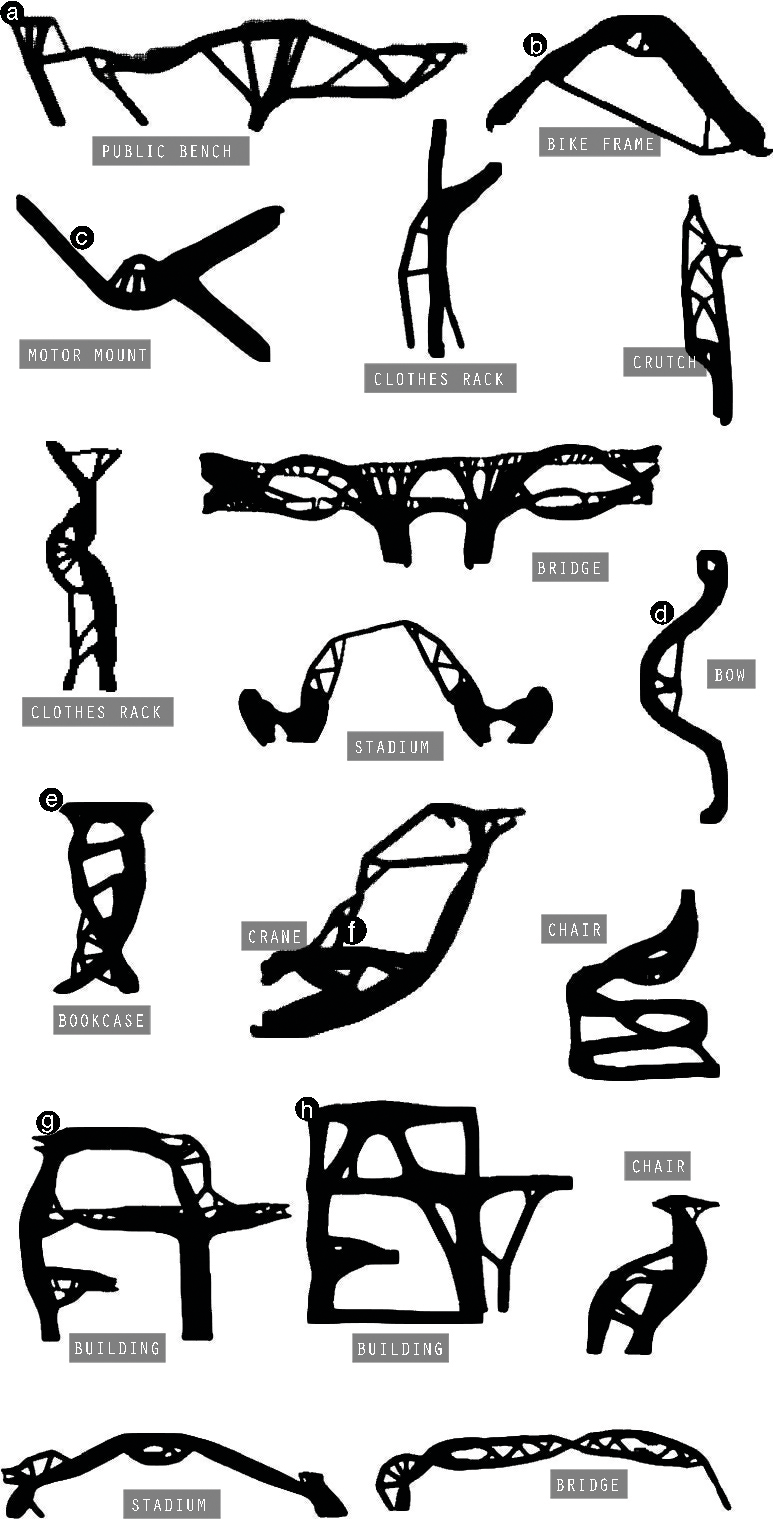
\includegraphics[width=0.6\textwidth]{figures/participants_design}
 \caption{Designs created by 10 participants using Forte.}~\label{fig:participants_design}
\end{figure}


\section{Post-processing and Fabricated Results}
Forte enables users to formulate, express and optimize their design in a 2D environment. To  fabricate their designs into 3D artifacts, we describe three post-processing techniques using external tools (e.g., the Rhinoceros\footnote{\url{https://www.rhino3d.com/}} CAD system) for fabrication and showcase some of the fabricated results.

\begin{figure} [h!]
  \centering
  \vskip 8pt
  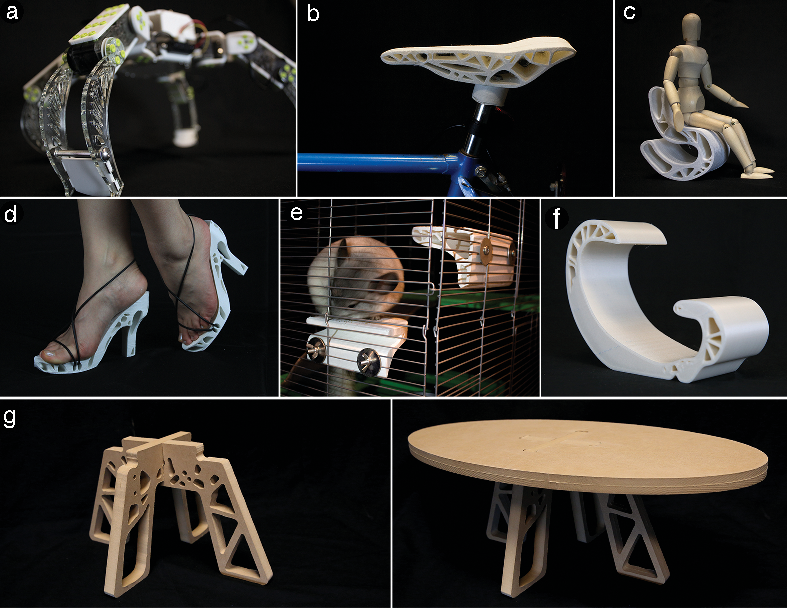
\includegraphics[width=1\textwidth]{figures/result_collage}
  \caption{Fabricated examples designed from Forte's generated structures: legs for a quadruped robot (a); a bike seat (b); an S-shaped chair (c); high heels (d); pet jumping platforms (e); a reading chair (f); and a tea table (g).}~\label{fig:result_collage}
\end{figure}


\begin{figure*} [t]
  \centering
  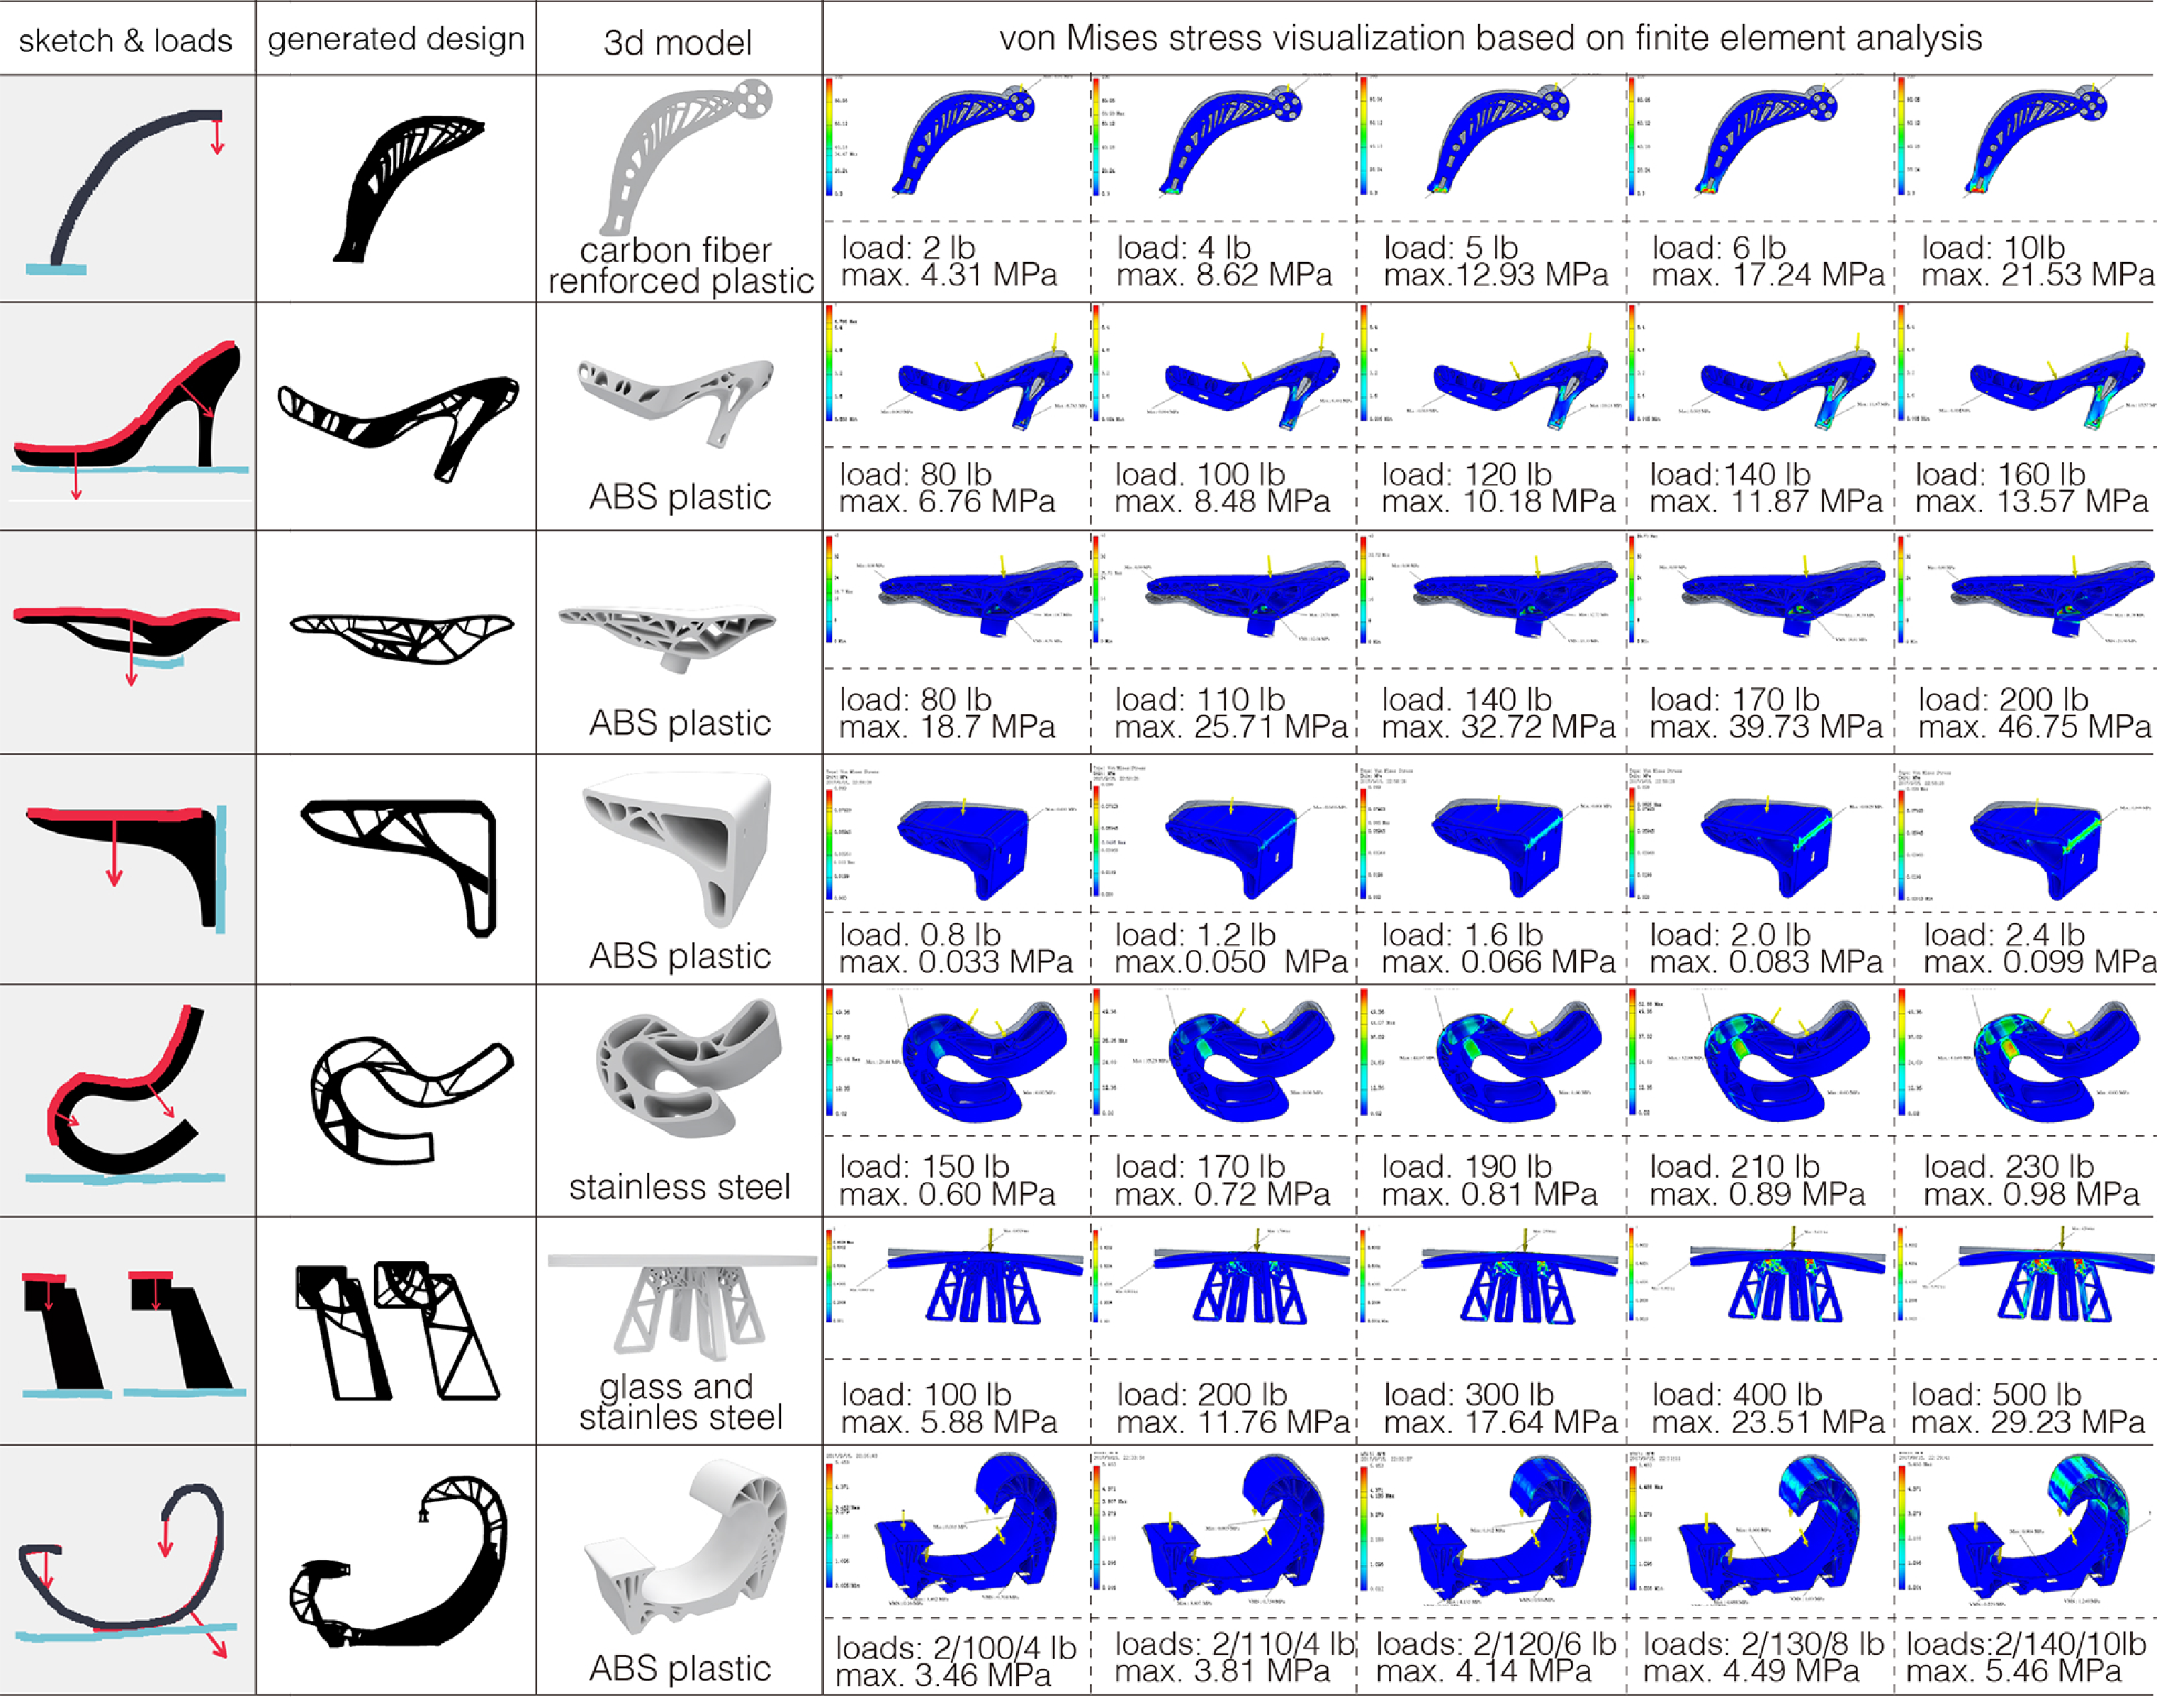
\includegraphics[width=1\textwidth]{figures/results}
  \caption{All our fabricated examples from the sketches in Forte, to generated 2D designs, and to post-processed 3D models; we performed a Finite Element Analysis on each 3D model based on the input loading scenario, which shows consistent stress distribution across a range of increasing loads.}~\label{fig:results}
\end{figure*}

\textbf{Extrusion} We can extrude a 2D design along a path to create a 3D object. First we convert a generated design from a bitmap to a vector graphic, which can already be used in a laser cutter to create planar objects, such as the legs for the quadruped robot (Figure~\ref{fig:result_collage}a). Further we can also import the vector graphics to a 3D modeling tool for creating a 2D surface and extruding it to a 3D object. We use this technique to create a multi-functional reading chair that consists of an overhead light, a reclined sitting area, and bookshelves (Figure~\ref{fig:result_collage}f). Extrusion is not limited to a perpendicular path: for example, it is possible to extrude the 2D chair profile in Figure~\ref{fig:result_collage}c along a circular path to create a bench.

% robot leg
% reading chair

\textbf{Warping} We can also warp a 2D design into a 3D surface. We used this technique to design a pair of high heel shoes using generated structures as the base (Figure~\ref{fig:result_collage}d). We designed a jumping platform for chinchillas by warping the cross-section to form a rounder top (Figure~\ref{fig:result_collage}e). We designed a bike seat by warping a 2D generated pattern to the shape of a cushion (Figure~\ref{fig:result_collage}b).

% high heel shoes
% chinchilla platform
% bike seat

\textbf{Combination} We can join multiple planar components made from the 2D designs (e.g., fabricated using laser or CNC cutting) to create 3D structures. For example, we designed a tea table supported by two joined structures (Figure~\ref{fig:result_collage}g).
%This cup holder mounted on an arm rest is made from two different generated components combined together.

% cup holder
% coffee table



To test the structural integrity of the 3D models produced in the post-processing step, we performed Finite Element Analysis (FEA) using Autodesk Inventor \cite{AboutSha59:online}. As shown in Figure~\ref{fig:results}, we tested each model on a range of increasing loads---from normal to overloading---and found consistent stress distribution across all the cases with high structural performance\footnote{We define the range of loads based on the usage scenarios of each design. The heatmap visualization is based on the maximum stress amongst all five loads.}. As our current focus is on the 2D design tool, this test is only based on our current examples (as well as specific types of material chosen for running FEA). Further experiments are required in order to validate the general process of converting 2D structural patterns to 3D objects manufactured in a wide range of materials, which we leave as future work.

% \begin{figure} [h]
%   \centering
%   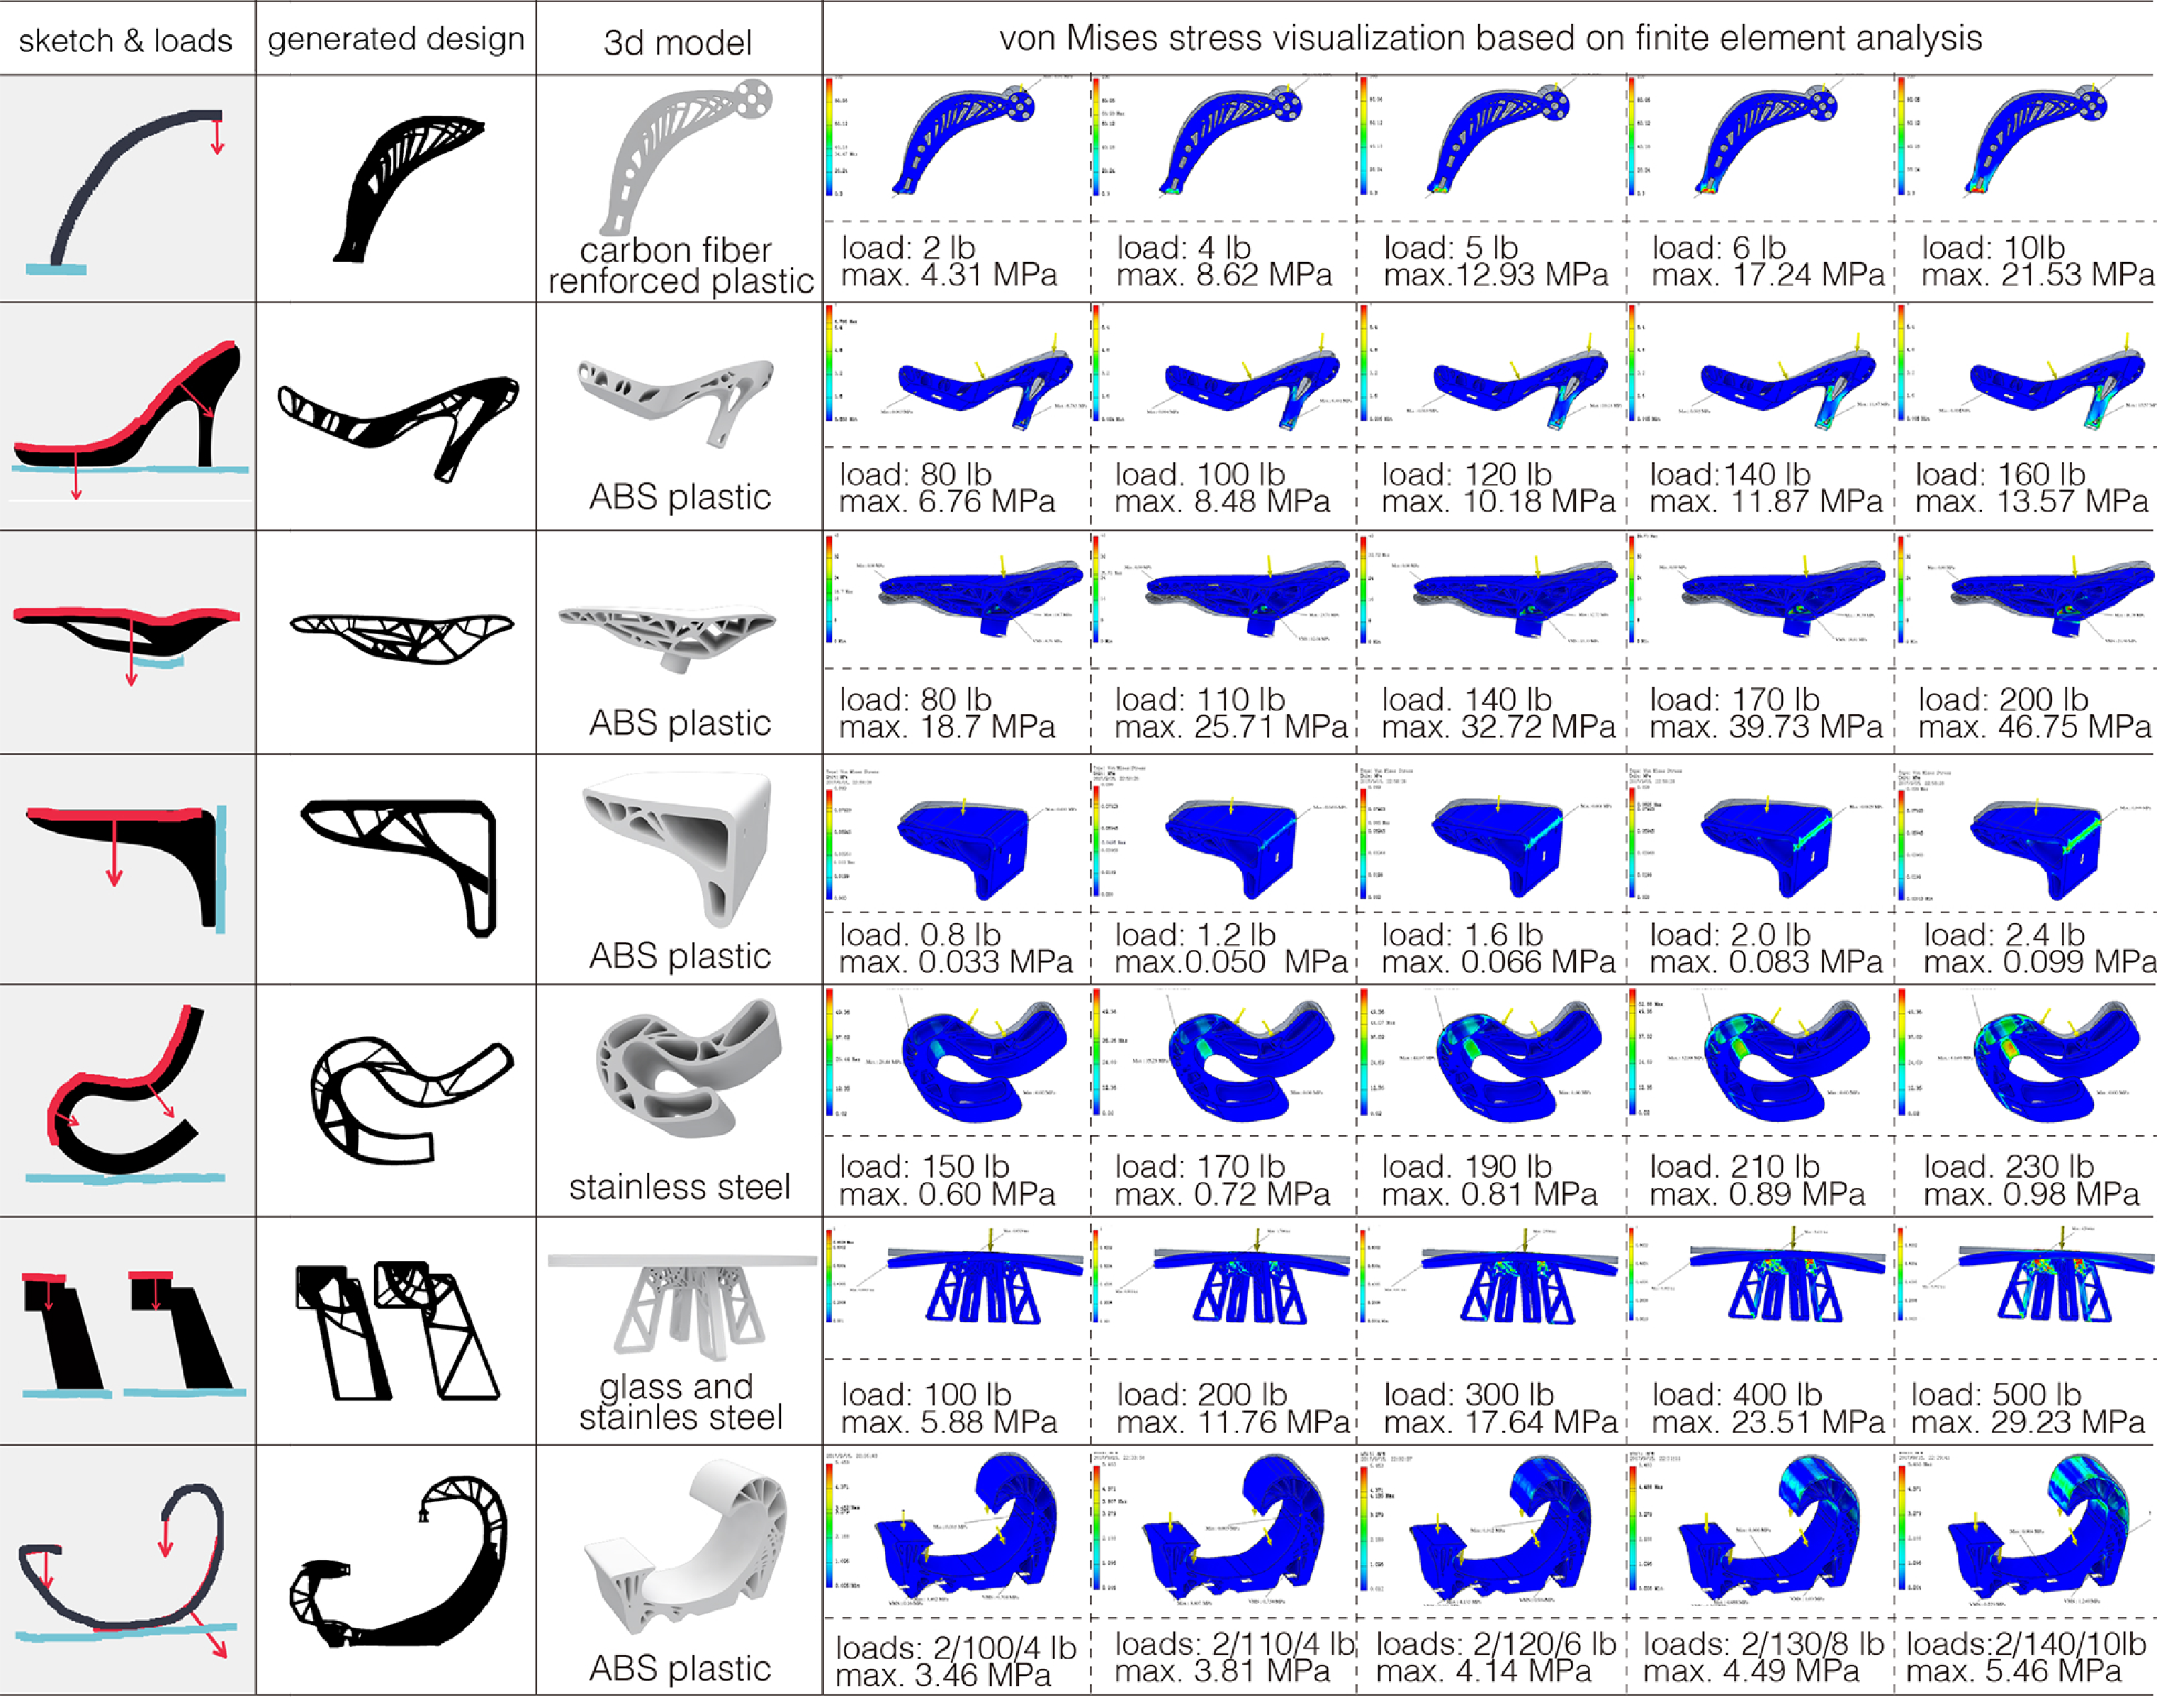
\includegraphics[width=1\columnwidth]{figures/results}
%   \caption{caption to be added.}~\label{fig:result_collage}
% \end{figure}
 
\section{Limitations, Trade-offs and Future Work}
We discuss limitations and trade-offs to better understand our current system, as well as pointing to potential future work.

\textbf{Going from 2D to 3D}
Forte is currently a 2D oriented tool, although our examples have shown three ways of extending it to 3D: extrusion, warping and combination. The implementation of Forte is also extensible to 3D: on the front end, prior work has demonstrated numerous techniques for enabling sketching in 3D \cite{igarashi2007teddy, bae2008ilovesketch, bae2009everybodylovessketch}; on the back end, the optimization can also handle 3D cases by adding a third dimension to the input parameters (design domain, loads, boundary conditions, etc.) as well as the material stiffness matrix. Perhaps the real challenge of going 3D is maintaining real-time feedback and interactive iteration. Past work has explored engineering solutions for handling 3D generative designs. For example, Aage et al. provide a topology optimization implementation based on PETSc (Portable and Extendable Toolkit for Scientific Computing), which enables incredibly fine discretization, e.g., a (3D) design with 27.6 million design elements running on 24 CPUs (144 cores) only requires 30-60s per iteration \cite{aage2014topology}. Building upon all this prior work, our next step will develop and extend Forte to a fully 3D design tool.

\textbf{Ambiguity and imprecision of sketching}
As mentioned in Gross and Do's work, sketching is a particularly appealing medium for early ideation and design formation, as it embraces ambiguity and imagination. As discussed in the design session, this is also a strength of Forte, as it allowed participants to use unique hand-drawn forms to generate structures. However, as pointed out by a few participants, Forte lacks support for more precise design, e.g., straight lines, smooth curves, and symmetry. In the future versions of Forte, we would like to add more controlled ways of specifying designs.

\textbf{Generating and exploring a large space of examples}
Currently each of Forte's optimized result is initiated and driven by the users. While this gives users freedom to explore and customize each optimization trial, it becomes a somewhat tedious process as the number of trial increases. In the future we plan to explore ways to automatically generate a large design space of structures from a single user input. To realize this, the challenge is two-fold: {\em(i)} how to infer and sample more variables from one single user input in order to generate more than one result; {\em(ii)} how to enable users to efficiently navigate and filter a large number of results. Our future work will explore solutions to tackle these two challenges.

\textbf{Enabling more semantic controls of design optimization}
On the input side, we are interested in enabling more semantic controls of design optimization beyond the similarity value. For example, in Yumer et al.'s work \cite{yumer2015semantic} they developed a number of semantic metrics for 3D models by having the crowd perform pair-wise comparison on a large data set. In the future, we want to let users label and quantify each optimization result, e.g., `how organic is this bike frame' and `how thin or muscular is this chair'. By collecting these quantified labels, we hope to map the space of the input parameters (e.g., amount of material, similarity, clearance) to the semantic space of the optimization outcome. This can potentially enable the `transfer' of design, e.g., applying a set of input parameters from an organic-looking bike frame design to turn this chair into a similar style.





%%%%%%%%%%%%%%%%%%%%%%%%%%%%%%%%%%%%%%%%%%%%%%%%%%%%%%%%%%%%%%%%%%%%%%%%%%%%%%%%%%%%%%%%%%%%%%%%%%%%%%%%%%%%

% one popular approach is to employ topology optimization \cite{bendsoe2013topology}---a well-established practice in mechanical and civil engineering. Essentially, topology optimization `automates' the design process by reducing the design input to only the functional requirements, e.g., overall size, amount of material, weight of loads, how the object is affixed to the world. The method then attempts to generate the strongest possible design given all these parameters as constraints. Although it gives functional assurance, from an HCI standpoint, topology optimization is too much of a `black box' that gives users very little control of expressing or editing their own design.

% In my ongoing work, I want to combine the best parts of both worlds: enabling users to sketch functional objects of their design by bootstrapping the process with topology optimization to transform the design into a functional one. Meanwhile, users will also receive step-by-step feedback and suggestion that connects the two worlds: as they create or edit their work, visualization informs them how the functionality is changing and what are the options to tweak the current design while staying with constraints. This mixed-initiative approach allows the system to assist users with their design task without limiting their freedom of creating or editing the object. As a result, users can benefit from delegating the functional aspects of design to the system while focusing on the visual appearance and styles. I hope such a design environment can help people fabricate a variety of things that meet real world requirements without requiring too much expertise from the user.

% There are several expected challenges in realizing this mixed-initiative approach, which are discussed in depth by Horvitz \cite{horvitz1999principles}. Foremost, there are many possible ways for a tool to combine user and system initiative. How much control shall the tool keep for the user and give away to the system? How can the user communicate their intent to the system and the system communicate its intelligence to the user? How can the system `merge' the two ends, resolve potential conflicts and finally achieve a result better than what the user (or the system) alone can achieve?

% \xac{moved original review to Ch2; added a few more optimization-specific works, which are more appropriate in this context}
% As reviewed in Chapter 2, prior work has explored guided design to help users achieve functional validity while designing geometry of objects. Specifically related to topology optimization, Christiansen et al. develop a tool to fully automate the design process from specifying input parameters (loads, boundary, objective, etc., which is detailed later in the chapter) to generating a functionally valid result that can then be fabricated \cite{christiansen2015combined}. However, it is somewhat unintuitive to start a design with functional consideration, rather than allowing users to describe their desired model to the system. Another challenging aspect of performing optimization is the scalability of performance. The demand for high resolution of the design will inevitably post challenges on interactive  tools. Wu et al. developed a scalable system using high-performance GPU-based solver to execute topology optimization, allowing million-scaled resolution \cite{wu2016system}. Although we can always expect future engineering effort to overcome today's performance issues, the development of design tools still need to keep in mind these potential performance challenges and constraints.

%  Building upon all this prior work, my research goal is to develop an end-to-end design tool with the following mixed-initiative work flow:

% %Prior work has explored guided design of functional objects. SketchChair allows a user to sketch a chair by drawing its cross section on a 2D canvas then `extruding' it to a full 3D model \cite{saul2011sketchchair}. Further, their tool can test the chair using a virtual human model and physical simulation, so that users are aware of any potential problem of their design \cite{saul2011sketchchair}. However, there is little support for informing the users how they could correct or improve their design. To bridge this gap, Umetani et al. propose a design enviroment that, during the geometric editing process, also continuously visualizes the valid range of the design parameters \cite{umetani2012guided}. Specifically, \textit{feedback} is provided to the users once a constraint is violated, while \textit{suggestions} guide them to transform the problematic design to a valid one. Although the system provides useful and executable guidelines, the design tasks seem to be fairly limited, primarily focusing on arranging a set of rectangular planks. Martinez et al. enables more freedom of expressing a visual pattern by providing a user-defined template \cite{martinez2015structure}. By feeding this template into an optimization pipeline, the system can achieve aesthetically pleasing design while staying close to a strong enough structure. Although these patterns define a user's desired appearance of the object, they remain as microscopic features; there is little support for users to design the macro geometry of the object other than indirectly providing functional constraints to the optimization pipeline.



% \begin{itemize}
% \item Enabling user to start with sketching or modeling a design from their intuition, without necessarily addressing any functional issues

% \item Next, guiding the user to go beyond the initial design and describe real world functional requirements, including
% \begin{itemize}
% 	\item how is the designed object situated in the real world?
% 	\item what is its spatial relationship with people and other real world objects?
% \end{itemize}

% \item Then users can iterate on the design back and forth between editing on their own and `handing over' the task to the system. Specifically, the user can edit their design based on a graph representation, while the system
% \begin{itemize}
% 	\item visualizes the `weak spots' - the stress of the design as a heat map rendered on the designed object
% 	\item computes a topologically optimized result given the functional constraints and the current design, which is then overlaid with the user's work as a way to inform them of potential changes to make to achieve a stronger structure.
% 	\item based on mechanical domain knowldege, provides a set of reinforcement solutions whereby users can select and apply to improve the current design
% \end{itemize}

% \item As the user becomes satisfied with the result, the system converts it into `fabricatable formats' that consist of 3D models of components and connectors to be assembled for the actual object.
% \end{itemize}

% As the work is still in progress, in this proposal I briefly describe several key components I envision of this project.

% \section{Sketching an Initial Design}
% Sketching is perhaps the most intuitive way of describing one's idea of a design, even for 3D objects. Igarashi et al. develop Teddy---a sketching interface whereby users, with a few 2D strokes, can create free form 3D models \cite{igarashi2007teddy}. Saul et al. applied a similar idea to designing chair: first drawing the 2D profile of the chair then `extruding' it for a complete 3D model \cite{saul2011sketchchair}. Through making a `rough' sketch to start a design, users are able to follow their intuition and creativity, rather than worrying about the detail or trying to overcome the general difficulty of creating 3D models.

% Thus the start-up interface of Mashup is no different than a familiar 2D sketch pad where users can create any freeform drawing representing an object they wish to design and fabricate.

% Next, Mashup converts the drawing into a graph representation that is amenable to further editing, enhancement, and the eventual requirement of fabrication. Essentially each drawn stroke becomes an $edge$, and incident edges are automatically joined by a $node$. At this stage, each edge is essentially a polygonal chain (or more commonly known as `polyline'); further iteration can add thickness along the edges and the nodes that connect them.

% \begin{figure*}[h]
% 	\centering
% 	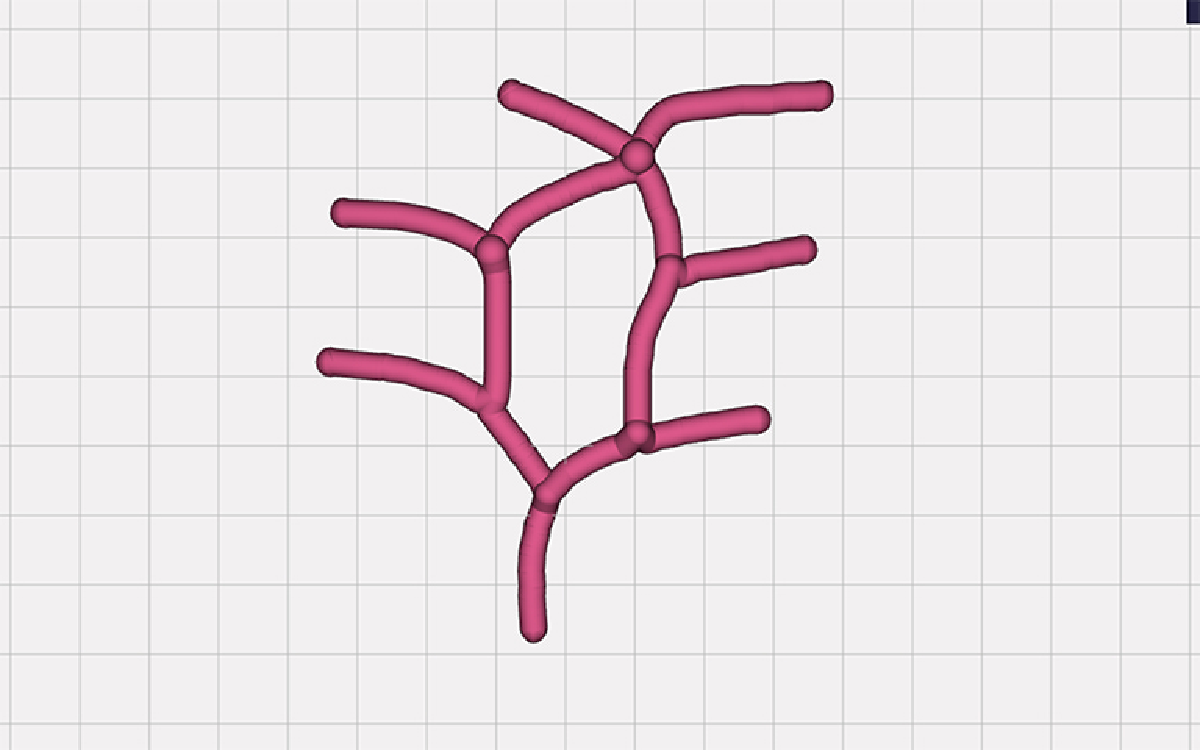
\includegraphics[width=0.8\textwidth]{figures/mashup_sketch}
% 	\caption{Users can start a design with sketching, such as this tree-like bookshelf.}
% \end{figure*}

% Such a representation is amenable to fabrication. Each edge will be fabricated as a mechanical component, such as a metal wire or a plank of wood; each node requires a connector that can accommodate all its edges; the thickness of the edges and nodes suggests the scale of these components and connectors. For example, an edge can be thickened to indicate the need of a wider or thicker plank of wood to strengthen the support. \xac{clarified?}

% Such a representation is also amenable to editing: once a sketch is created and converted to this representation, users can edit it by dragging and repositioning the nodes, removing nodes or edges, splitting an edge, or changing the thickness along an edge.

% Finally, both the sketch and the subsequent representation are extensible to 3D. Users can tilt the 2D canvas and sketch `out of the paper'. However, at any given time, users only need to deal with 2D sketching or editing, which is mapped to a 2D canvas automatically computed based on the users' viewing angle (i.e., the camera angle of the 3D scene). Alternatively, users can also `extrude' a 2D sketch along a third dimension to make it a 3D model, which is similar to the SketchChair's approach \cite{saul2011sketchchair}.

% \section{Specifying Functional Requirements}
% To design a functional object, a visual sketch is not enough to describe its functional requirement. As a next step, Mashup guides the users to transition from thinking of the design visually to considering and describing its functional aspects. One important functional aspect for many everyday objects is the ability to support themselves as well as other objects interacted with. Furniture is a class of such objects: step stools, chairs, tables, bookshelves, and clothes racks are just a few examples of objects that need to sustain things to be put on them or people to be sitting, standing or lying on them. Other examples include all kinds of bases, stands, holders, hooks, all of which are also required to support certain objects when deployed to use.

% \textbf{Loads} Mashup lets users specify these functional requirements in just a few steps. Specifically, as users finish the initial sketch, they can switch to the `functional specification' mode, in which they can click or tap on their drawing to specify where other objects or people might be situated, such as where books are placed on a bookshelf, where people stand on a step stool, and clothes are hung on a rack. This is called a \textit{loading point}. Next, Mashup infers the direction of the force exerted by the load, which can be computed by taking the normal of the sketch at the loading point. Users can then estimate the amount of load by adjusting a slider.

% \textbf{Margin} Further, to inform future iteration, some space on the original design needs to be allocated and kept empty so loading objects can be put in place, such as leaving enough space on a shelf to put on books of certain size, or clearing space above a step stool for people to step on. Such necessary empty space is called a \textbf{margin}. As shown later, marking margins prevents the system from mistakenly add extra components to the original design that might defeat users' original intent of usage. Margin can be specified immediately following a load: users can extend the loading point to a bounding box delineating the space of margin.

% \begin{figure*}[h]
% 	\centering
% 	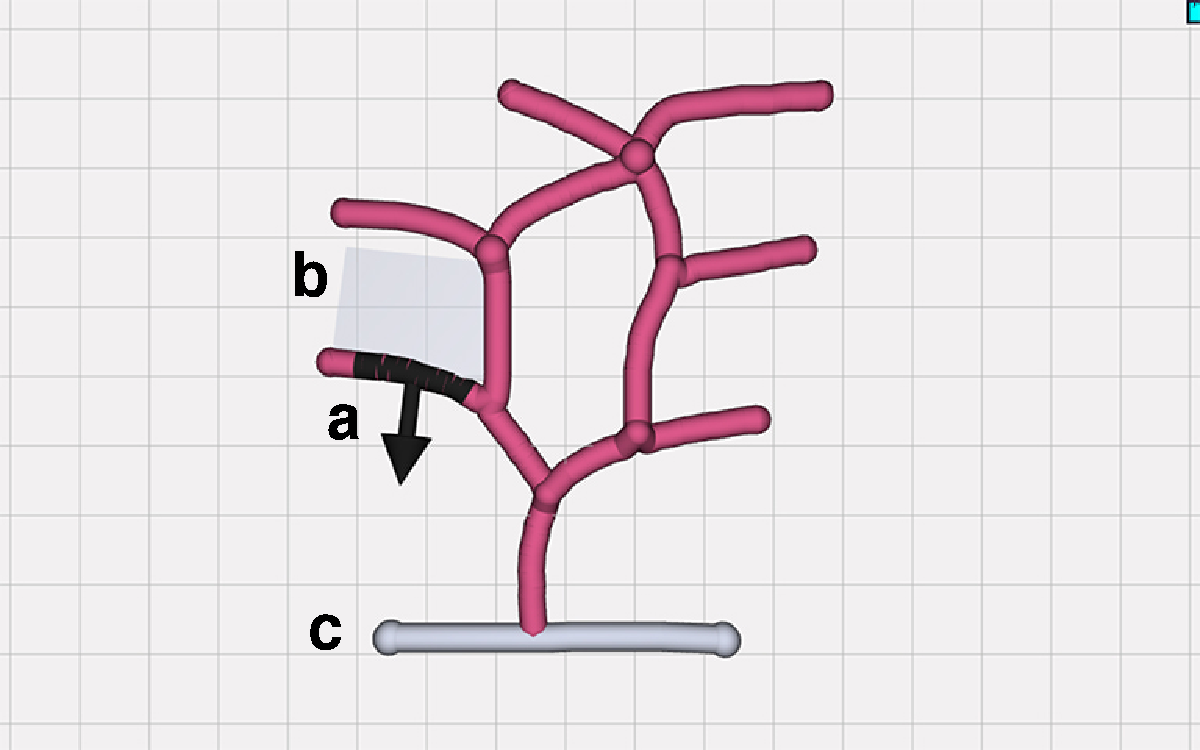
\includegraphics[width=0.8\textwidth]{figures/mashup_funcreq}
% 	\caption{As the next step, users specify functional requirement of the design, such as which part of the bookshelf will need to support books and what is the direction of the loading force (a). Some space should stay `empty' in order to place books (b). The bookshelf will be situated on and supported by the ground (c).}
% \end{figure*}

% \textbf{Boundary} Besides loads, another important piece of functional information has to do with how an object will be situated in the real world once fabricated. In many cases, objects will be placed on the ground or some horizontal surfaces, such as chairs, bookshelf, tables. Others might have different scenarios, such as a hook attached to the wall, a candle chandelier hung from the ceiling. These points of affixation are called the\textit{boundary} for the object. At points of boundary, forces will occur to counteract those exerted by the loads, such as the ground supporting a chair while a person puts their weight on it. Users can specify a boundary by first selecting a point on the sketched design, and then expanding it as a bounding box to encompass the size of boundary.

% At this step users have to go beyond the initial design and think more about the functional aspects of the object. Mashup seeks to make such functioal specification simplified to only a few steps, and closely associated with and based on the original sketch rather than having to describe it in purely abstract and technical terms.

% \section{Iterating a Design with System Feedback and Suggestions}
% Although at this point users have provided functional requirements of the object in design, making sure that the design satisfies these requirements would still demand expertise that might go beyond everyday users. Thus, as the users iterate on their initial design, Mashup wants to bring in computational support through which the system might take various degree of initiative to help the users enhance the functional aspects of their design. Primarily, Mashup provides users with \textit{feedback} that shows the `goodness' of the current design and highlights problematic parts. Mashup also offer \textit{suggestion} that informs users how they can strengthen the design to better meet the functional requirements.

% \subsection{Analysis and Feedback}
% Mashup's feedback is primarily based on a finite element analysis (FEA) of users' design and the functional requirements they have specified. In short, FEA discretizes a design into connected elements (e.g., a voxel grid) and analyzes their behavior given the intrinsic geometry and the external forces (e.g., loads).

% \xac{more explanation of FEA here}
% One useful metric computed from FEA is the \textit{displacement} of the design's constituent elements. Microscopically, this metric indicates how an element will move given all the design parameters; macroscopically, displacements of elements can jointly reveal how the object in the design will react to an actual usage scenario, such as collapsing under loads, or toppling due to imbalance. A global displacement vector $U$ (consisting of displacements of all the elements) is governed by the following relationship:

% \begin{equation}
% \mathbf{F} = \mathbf{K}\mathbf{U}
% \label{eq:forcedisplacement}
% \end{equation}

% $F$ is the global force vector. $K$ is the global stiffness matrix, which is dictated by the material property of the object. \xac{non-minor revision here:} Specifically, the discretized design consists of interconnected nodes (for voxels, each voxel has eight nodes that are also connected to other voxels). To obtain displacement vector on each node, we need to solve Equation~\ref{eq:forcedisplacement} to obtain $U$. $F$ is already given from user-specified load. To obtain $K$, we will go through each element $e$, retrieve its nodes, and add to them the stiffness matrix of $e$.

% Once displacement is computed, Mashup visualizes it as an overlay atop the users' design. Instead of overwhelming users with visual details, Mashup combines the displacements of each elements to `global arrows' showing potential movement of entire object under the specified loads.

% While displacement shows the result of a design given external loads, it does not necessarily indicate the causes of such displacement. For example, if a branch of a clothes rack bends under the weight of clothes, the cause is often not at the tip that displaces the most, but rather at the bottom or branching points due a lack of support. Thus Mashup also computes \textit{stress}---a metric that is more useful in identifying where structural problems can be mitigated. Similar to displacement, stress is also computed in an element-wise manner. At element $e$, assume $v_1$, $v_2$ and $v_3$ are vectors from this element to three of its connected neighbors. Correspondingly, $V_1$, $V_2$ and $V_3$ are vectors after the displacement. First, we compute a transformation matrix $F$ that describes the spatial relationship between these two sets of vectors:

% \begin{equation}
% F[v_1, v_2, v_3] = [V_1, V_2, V_3]
% \end{equation}

% With $F$, we can then compute the Green strain:

% \begin{equation}
% E = {1\over2}(F^TF-I)
% \end{equation}

% By taking the Frobenius norm\footnote{A Frobenius norm of matrix $A$ is square root of the sum of the absolute squares of its elements.} of $E$ we can obtain a value that indicates the stress of the element. To visualize this information, Mashup creates a heatmap rendered over the users' design. Internal elements by default are not visible. To visualize them the heatmap is rendered with transparency. Users can also `slice' an object open to view the internal visualization.

% \subsection{Optimization and Suggestion}
% Although feedback informs users of problems of their design, it does not provide solutions. As such, Mashup can translate the analysis results from the previous step to actionable suggestions that will guide users to modify and enhance their design in a problem-solving manner.

% The first approach for suggestion is to provide a built-in collection of ad hoc solutions and to apply them to the current design instance. For example, a rule of thumb for strengthening a weak spot of an object is simply to make it larger in volume. To support a horizontal structure, we can always connect overhanging parts to portions of an object below that structure. Mashup will allow users to choose from these ad hoc solutions, which are then automatically parameterized, generated and attached to the user's design. Although these small fixes are easy to understand and deploy, they might not effectively solve the design problems---even worse, they might cause new problems while trying to solve an existing one. For example, thickening one part of an object might cause a global imbalance problem. To address this issue, Mashup performs an FEA of the new design in the background as users apply these ad hoc solutions, and visualizes how the solutions are solving problems or causing new ones. Mashup also lets users apply solutions in a `suggested editing' mode, whereby changes are tracked and easily reversible.

% In addition to the ad hoc solutions that attempt to fix problems locally, Mashup can also performs a global topology optimization, which generates the strongest possible design given all the specified constraints. In short, given a design domain (e.g., the bounding volume of a bookshelf), the functional requirements (loads, margins and boundaries) and the available amount of material, topology optimization comes up with a structure within the design domain that yields the least compliance (i.e., can best sustain the loads with the least amount of deformation). Through the optimization process, a design is achieved by selectively removing elements from the design domain. Based on the summary by Sigmund \cite{sigmund200199}, the process can be formalized as follows:

% %\begin{multline*}
% %\end{multline*}

% \begin{equation}
% 	\min_x: c(\mathbf{x}) = \mathbf{U}^T\mathbf{K}\mathbf{U} = \sum^N_{e=1} (x_e)^p\mathbf{u}_e^T\mathbf{k}_e\mathbf{u}_e,\\
% \end{equation}

% 	subject to

% \begin{gather*}
% 	{V(\mathbf{x}) \over V_0} \leq f \\
% 	\mathbf{K}\mathbf{U} = \mathbf{F} \\
% 	0 < x_{min} \leq x_e \leq 1
% \end{gather*}

% As with the FEA for analyzing displacement, $\mathbf{U}$ is the global displacement vector, $\mathbf{F}$ is the global force vector, and $\mathbf{K}$ is the global stiffness matrix. $\mathbf{u_e}$ and $\mathbf{k_e}$ are the displacement and force of element $e$, respectively. $\mathbf{x}$ is the vector of design variables: for a design discretized into $N$ elements, $\mathbf{x}$ is an $N$-tuple vector with $x_e$ representing the density of element $e$---the smaller value of density means the more likely this element will be removed; and vice versa. ${V(\mathbf{x})/V_0} \leq f$ describes the constraint on the amount of material---it establishes a maximum percentage of the total material found in the design volume that is to be used in the solution.

% While this seems a nice `shortcut' to jump from the initial design to a potentially more functional one,  this approach does have some inherent limitations. Foremost, the optimization process by nature is only concerned with functional requirements. It has no knowledge of what the user would want the final result to look like. Thus as a preprocessing step, Mashup imports user's initial sketch into the optimization input variables, and marks those elements as non-removable. Effectively, this stipulates that the final optimization result must contain this initial design. In other words, the outcome of the optimization is additional structure to the user's original design to make it better fulfill the functional requirements.

% However, even with this user input, it might happen that the optimization process will add unwanted components that render the object unusable, such as components on top of a chair's sitting area. To prevent this from happening, Mashup also imports the previously specified margin areas to inform the optimization process that there are elements that must be removed, such as keeping the space above a chair's seat empty.

% \subsection{Iterating with User Editing}
% As the system optimizes user design additively, Mashup allows users to have control of how much extra material will be added. With the aforementioned real time feedback, they can interactively play with this variable to ensure that their design idea is retained while the object remains strong enough to fulfill the functional requirements.

% Users can also use their initial design as `seed' to intentionally generate variations---other functionally valid designs that are drawn but also deviate from their original ideas. At the system's level, this is achieved by controlling the `weight' of user's initial input---instead of treating these elements as absolutely non-removable, the system can variously loosen the constraint to generate a set of design variations for users to choose from.

% Users can also manually edit the object on their own by manipulating the `primitives'---the edges and nodes representing the design. They can adjust the length, thickness and position of each component, or add more reinforcement structures, such as a diagonal cross bar to better support a weak spot, or removing ones that no longer feeling needed. As they perform such manual editing, they can control how proactive and frequent the system responds to user's input: providing feedback and suggestions step by step, periodically, or on-demand.

% \section{Making a Design Fabricatable}
% As a final step, Mashup will convert users' design into something fabricatable. Previously, to simplify the design, users only provided a low-fidelity, skeletal profile of an object. To fabricate the design, Mashup allows the users to produce the design as one homogenous object or as separate parts to be assembled.

% \xac{non-minor revision on 2d/3d, CNC}
% To make it in one piece, Mashup joins all the `primitives' and generate a cross-sectional area with smoothed profile based on the thickness of the nodes and edges.  As a sketch might only represent a 2D profile of a 3D object, to actually fabricate it the users can simply extrude the 2D profile into a full 3D object. Mashup can either export the object as a 3D printable model, or as other formats, such as for using laser cutting or CNC milling of e.g., plywood sheets, can accommodate large creation, and requires Mashup to provide the size of the raw wood material and the number of cuts (as each time the machine can only cut through a limited depth of material).

% To make use of existing parts and assemble the object, users specify the raw components, such as Lego bricks, planks of wood or PVC pipes. Mashup then computes and generates a corresponding subset of these components, as well as instructions to put together to assemble the design. In some cases, Mashup also generates connectors for joining these components in specific ways (e.g., with specific angle and sufficient strength). When needed, Mashup also generates instructions for cutting the components if their original dimension exceeds what is required to compose the object.

% \section{Summary of Mixed-Initiative, Functionally-Aware Design}
% In contrast to Reprise's tasks of making adaptations attached to existing objects, Mashup attempts to produce standalone designs with functional relationships to real world objects. Specifically, it focuses on combining the requirement of supporting loads of these objects and the freedom for users to express their own design. This mixed-initiative approach brings everyday users further into the realm of functional fabrication without demanding much of expertise from them. In so doing, I hope we can expand the range of things everyday users can make. The next chapter will discuss further involving the users in the fabrication process, by supporting them in carrying out making tasks on their own.
